\subsection{Odległość od optimum}

Z~rys.~\ref{fig:avg} wynika, że~dla~każdej instancji problemu, heurystyka i~algorytmy przeszukiwania lokalnego osiągają podobne wyniki, które są~kilkukrotnie lepsze od~rozwiązania losowego, z~którego startują zarówno Greedy, jak~i~Steepest. Algorytmy Greedy i~Steepest dają podobne rezultaty --- różnią się nieznacznie dla~różnych instancji i~nie~ma~tendencji co~do~tego, który ogólnie działa lepiej. Można za~to~zaobserwować, że~oba~algorytmy przeszukiwania lokalnego są~lepsze niż~heurystyka.

\begin{figure}
\begin{center}
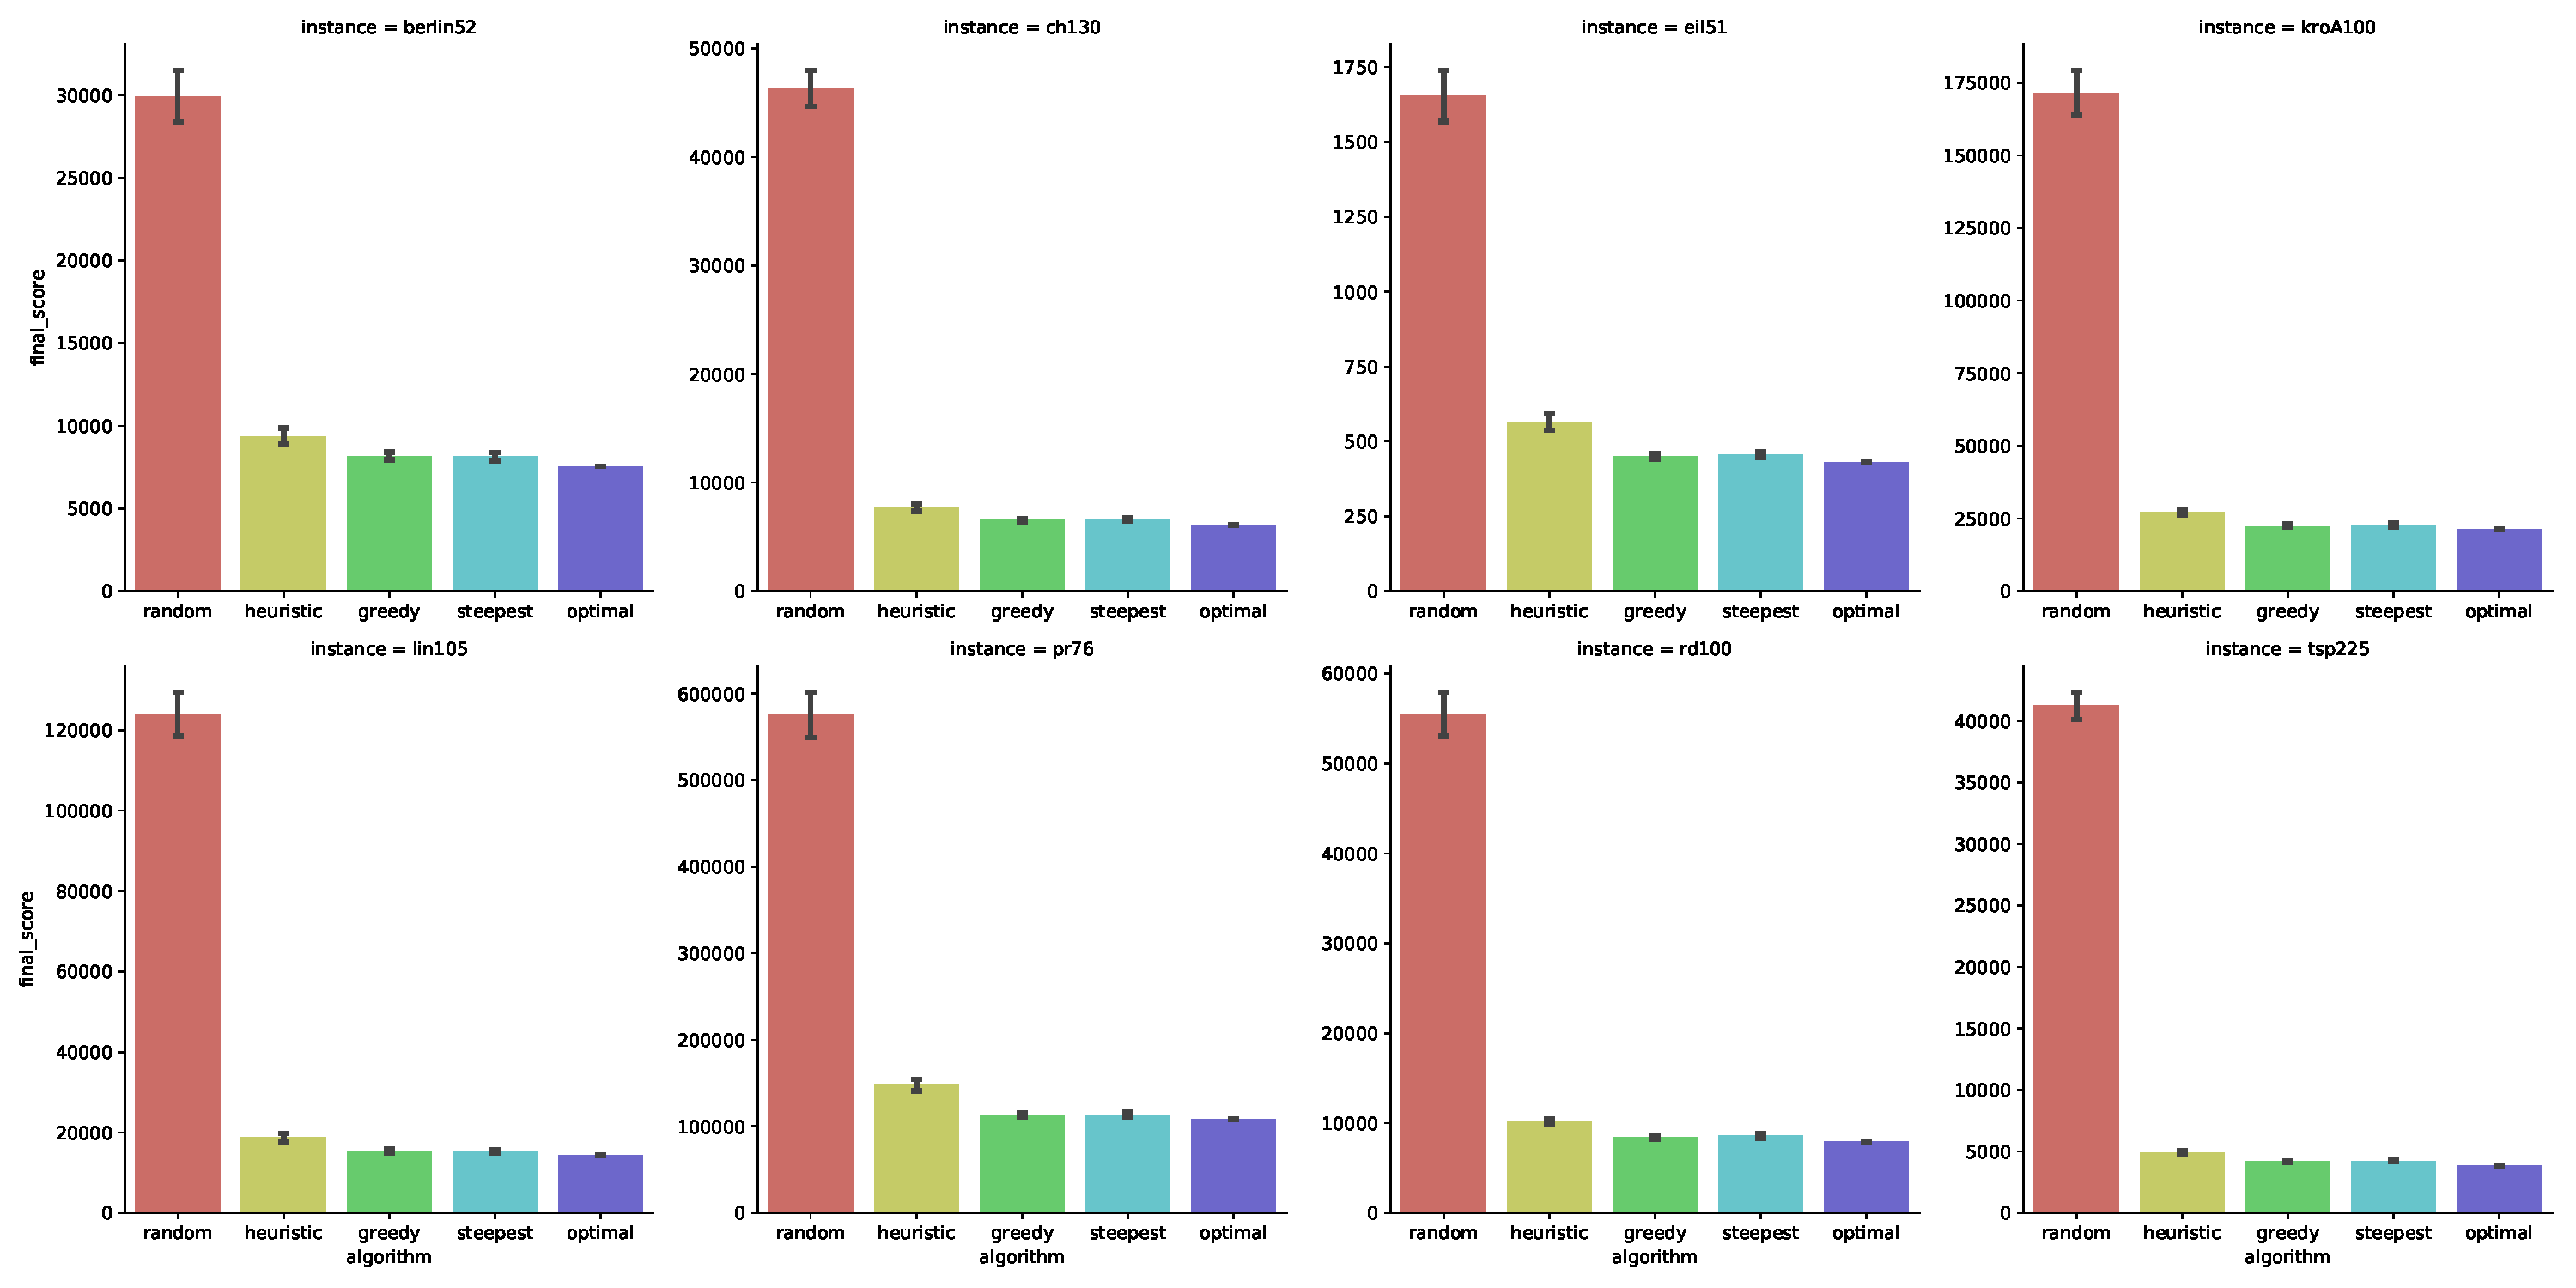
\includegraphics[width=1.0\textwidth]{graphs/score_comparison_bar_avg.pdf}
\end{center}
\caption{Porównanie średnich rozwiązań na~różnych instancjach.}
\label{fig:avg}
\end{figure}

\begin{figure}
\begin{center}
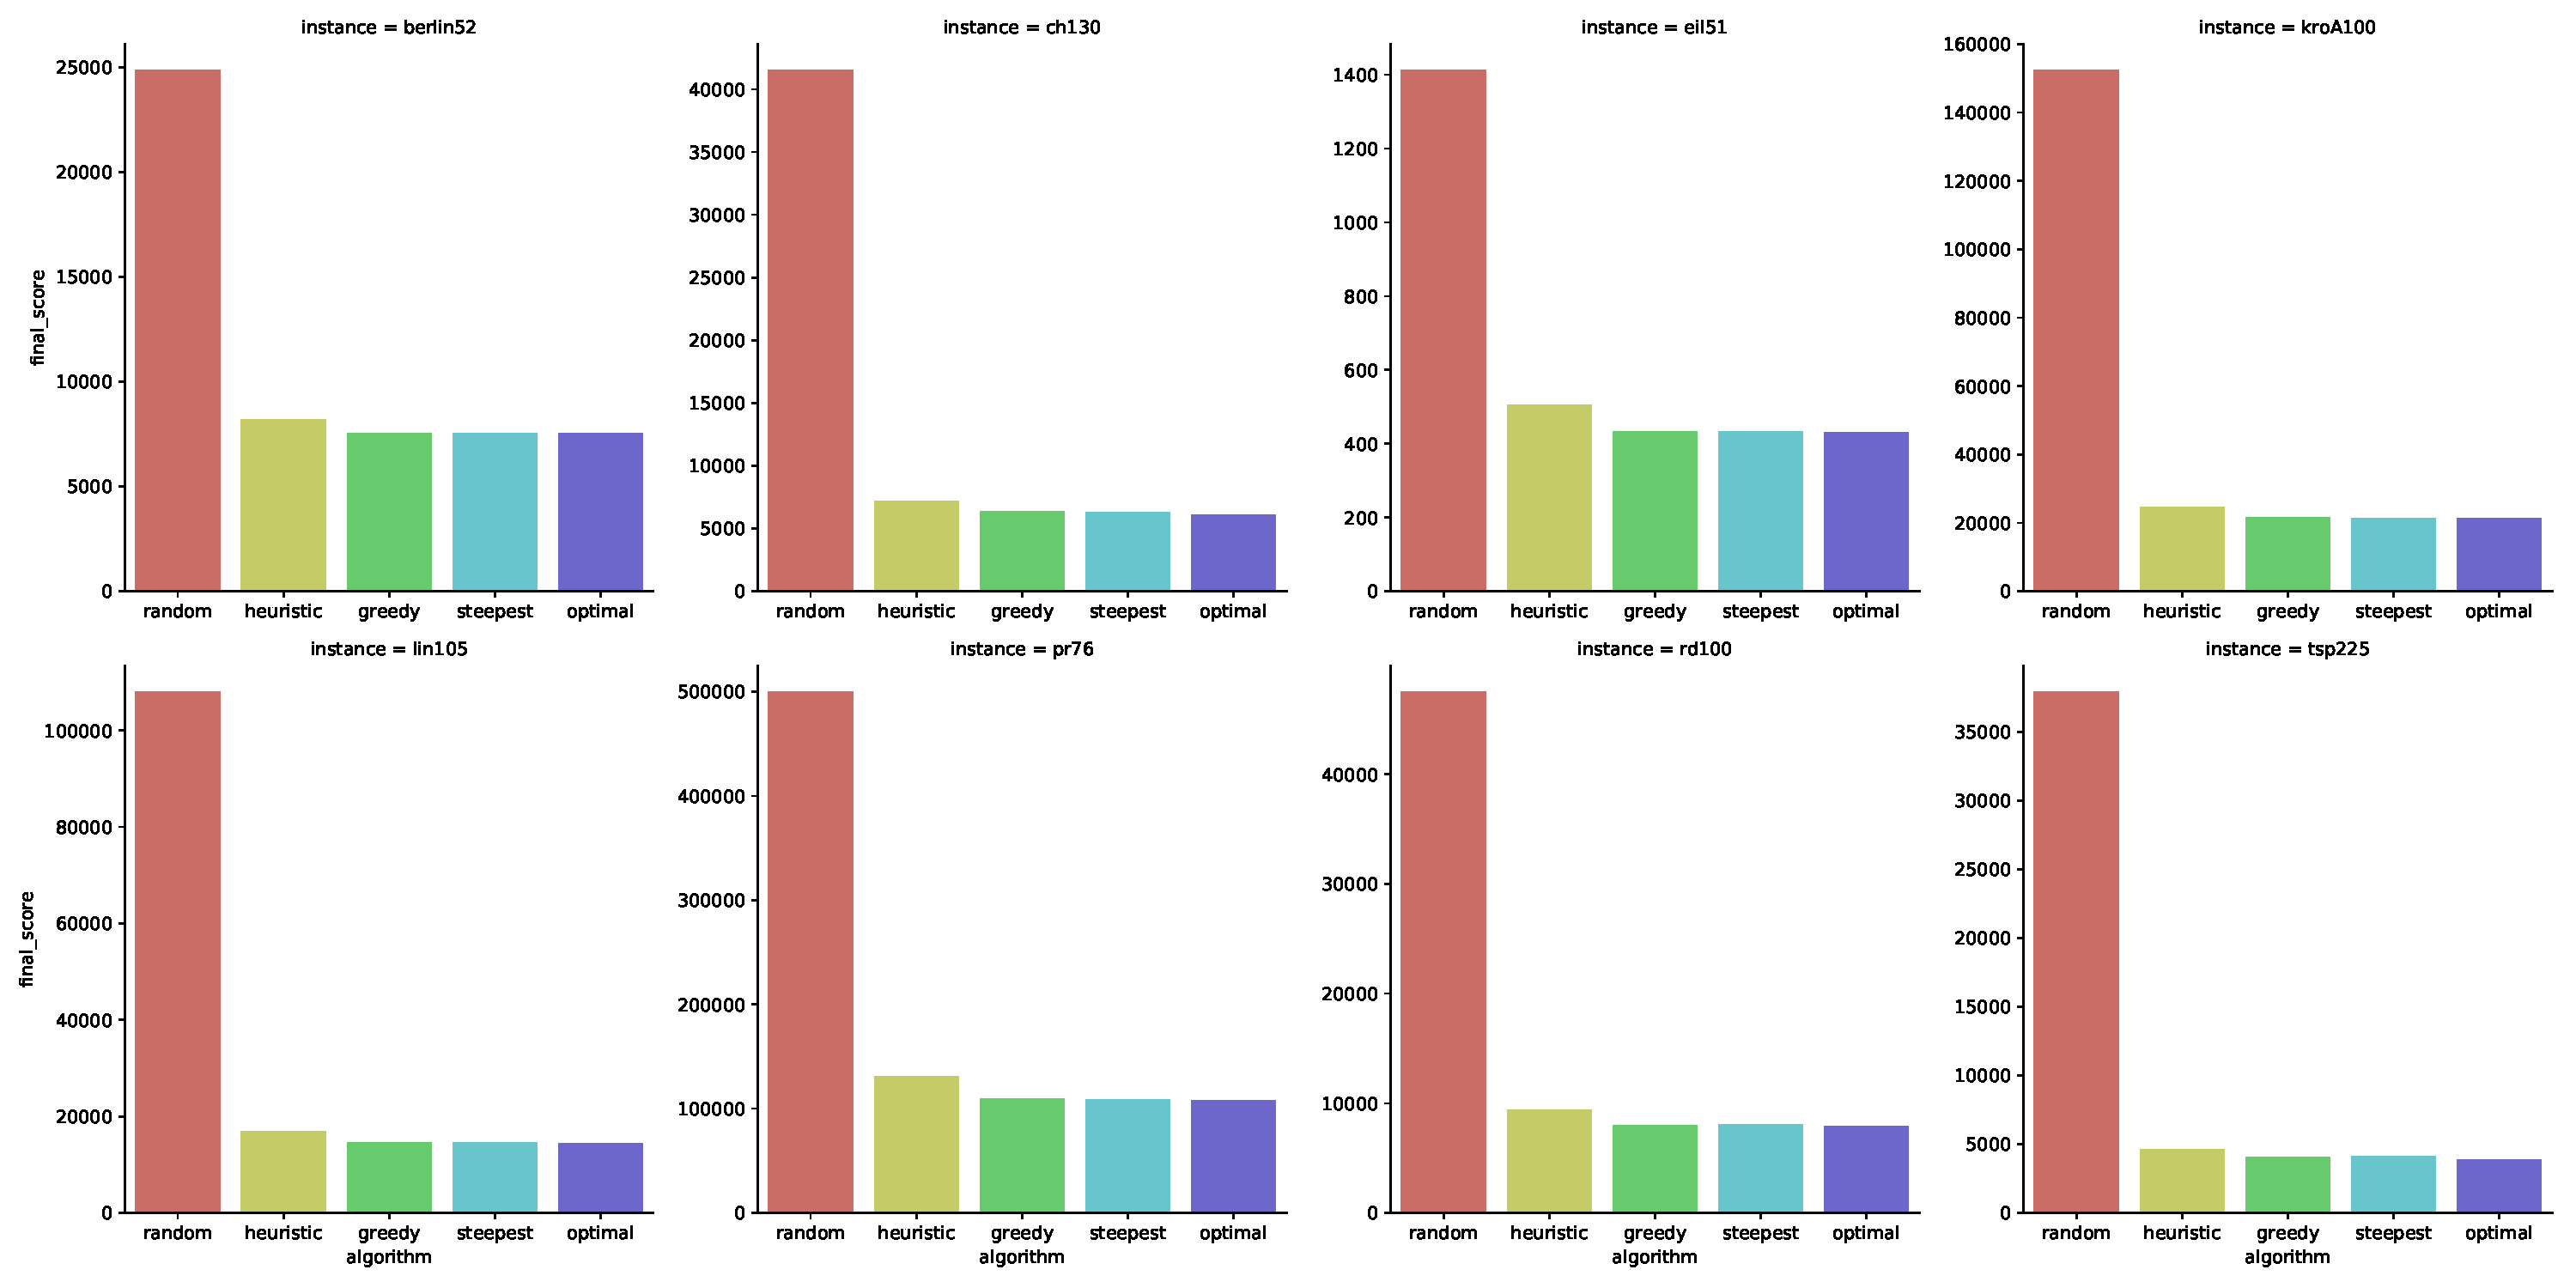
\includegraphics[width=1.0\textwidth]{graphs/score_comparison_bar_min.pdf}
\end{center}
\caption{Porównanie najlepszych znalezionych rozwiązań przez~algorytmy na~różnych instancjach.}
\label{fig:best}
\end{figure}

\begin{figure}
\begin{center}
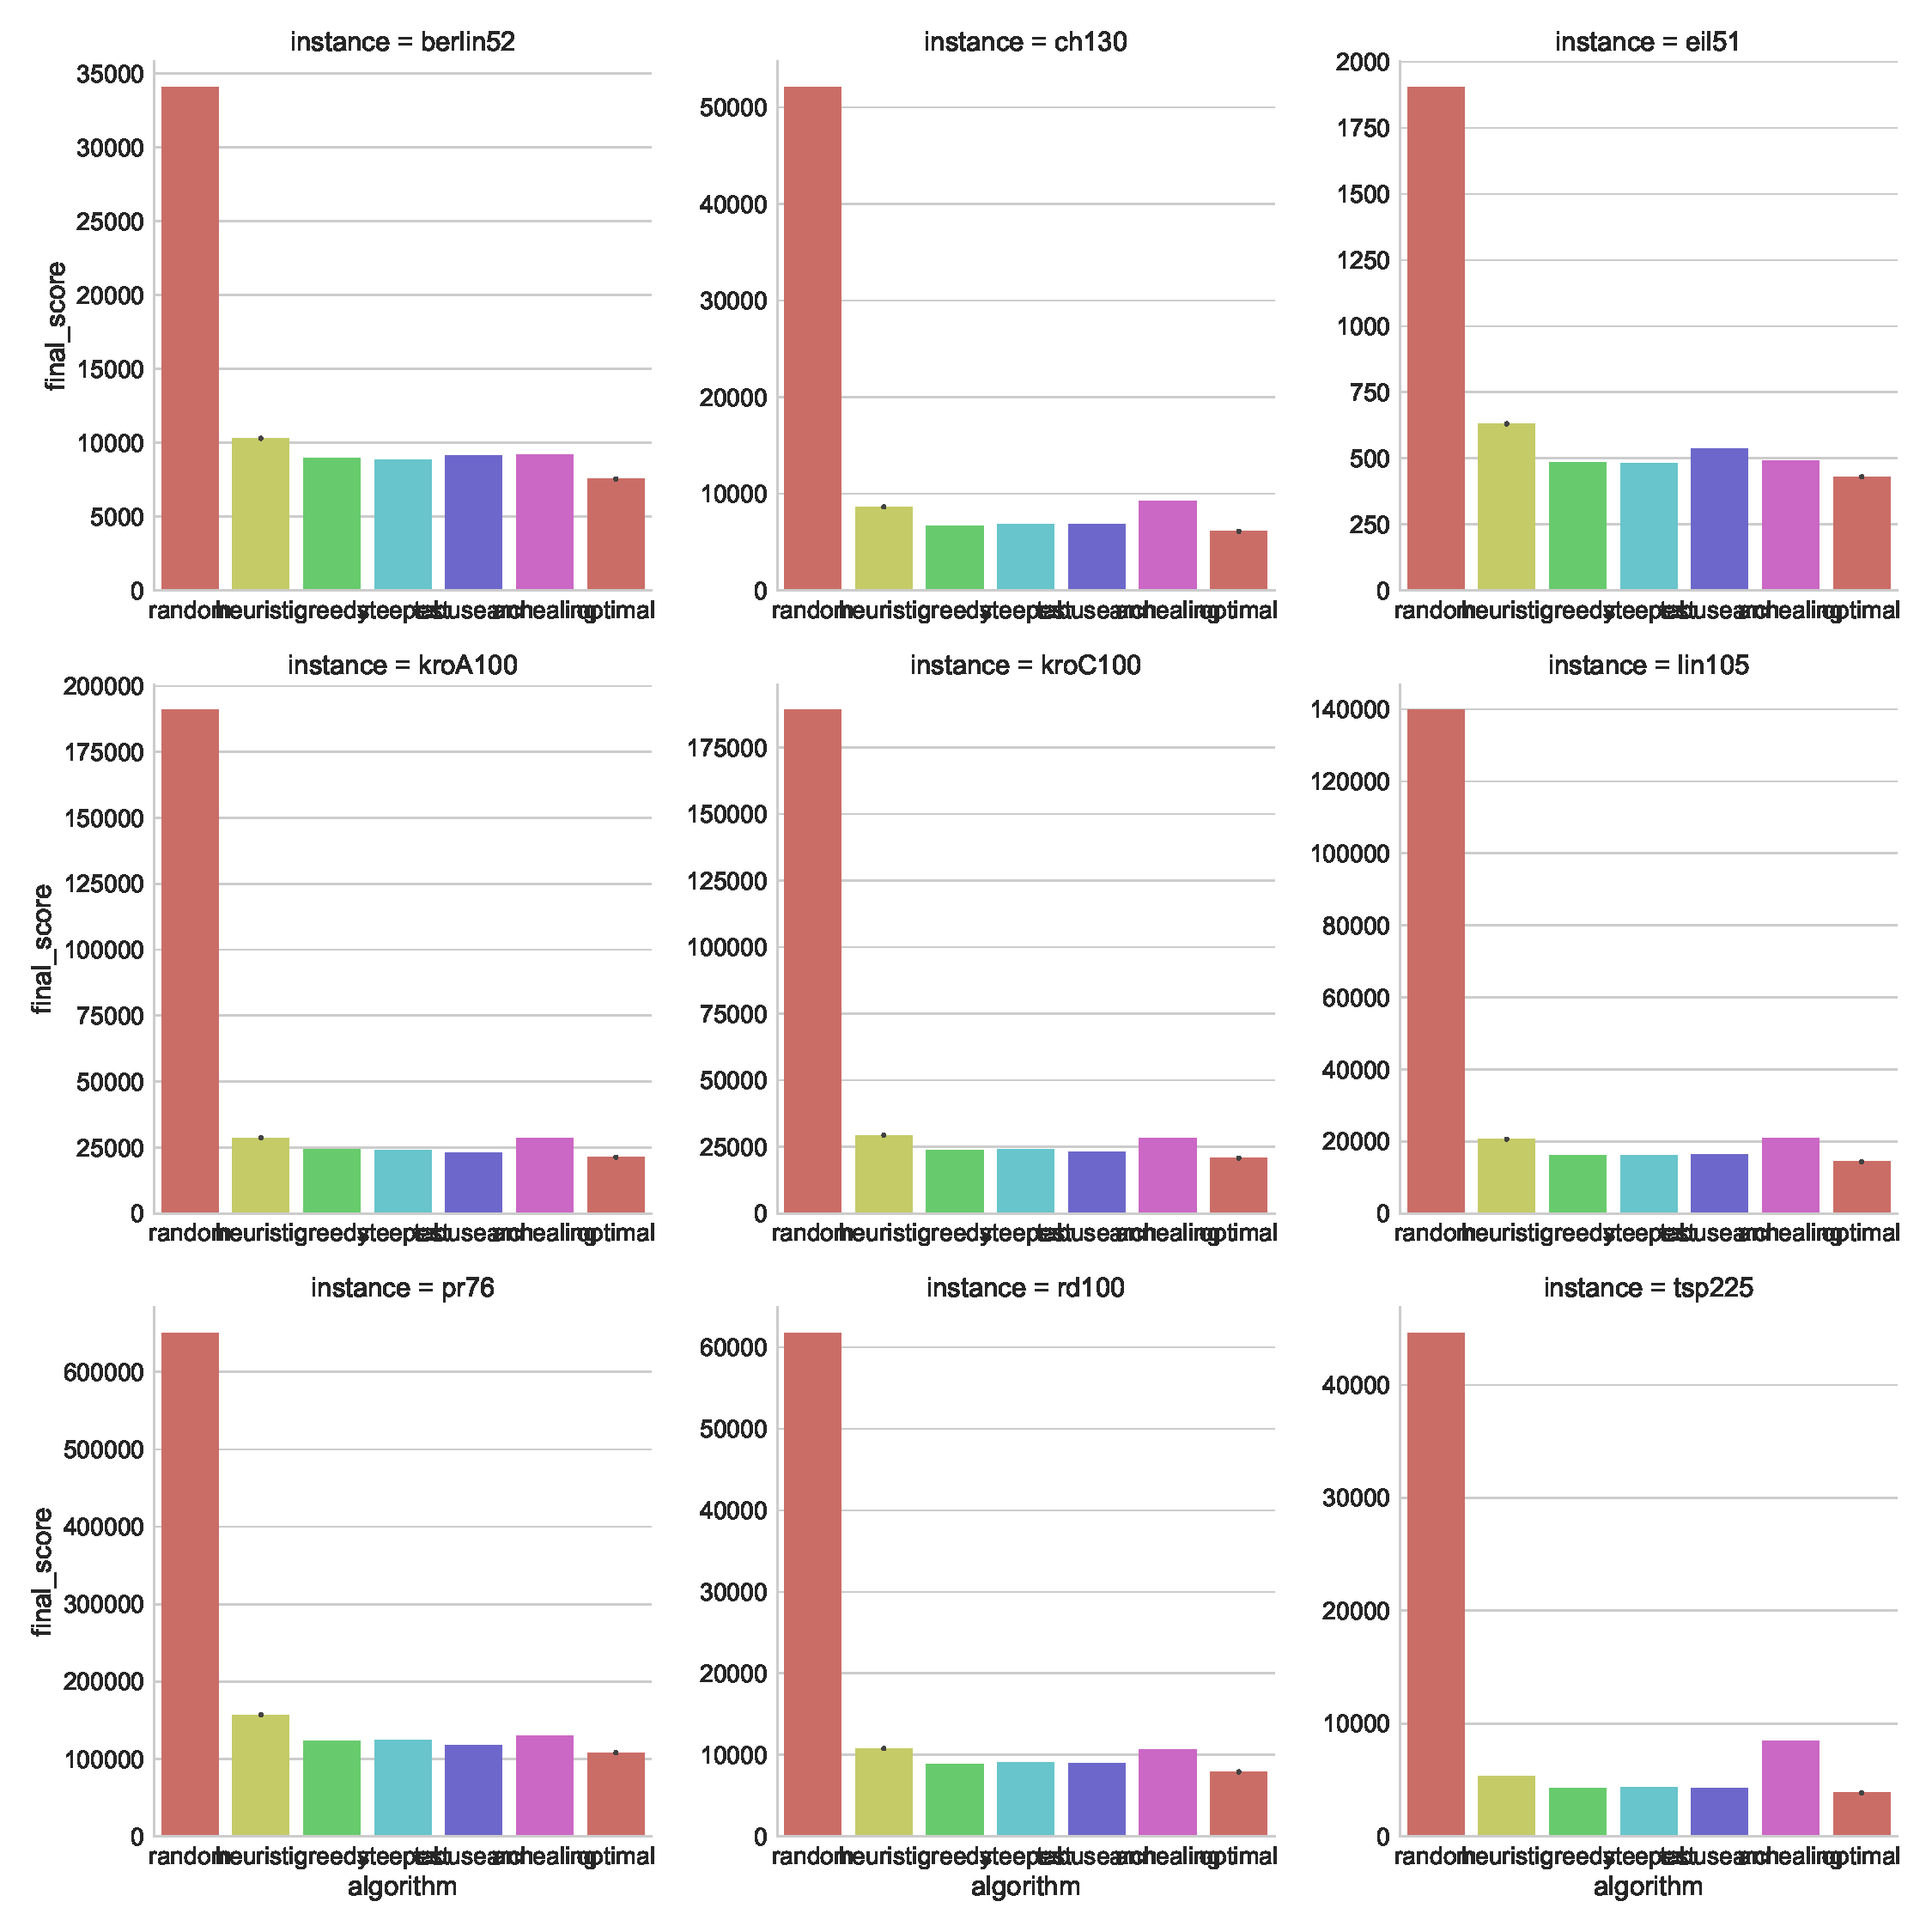
\includegraphics[width=1.0\textwidth]{graphs/score_comparison_bar_max.pdf}
\end{center}
\caption{Porównanie najgorszych znalezionych rozwiązań przez~algorytmy na~różnych instancjach.}
\label{fig:worst}
\end{figure}

\begin{figure}
\begin{center}
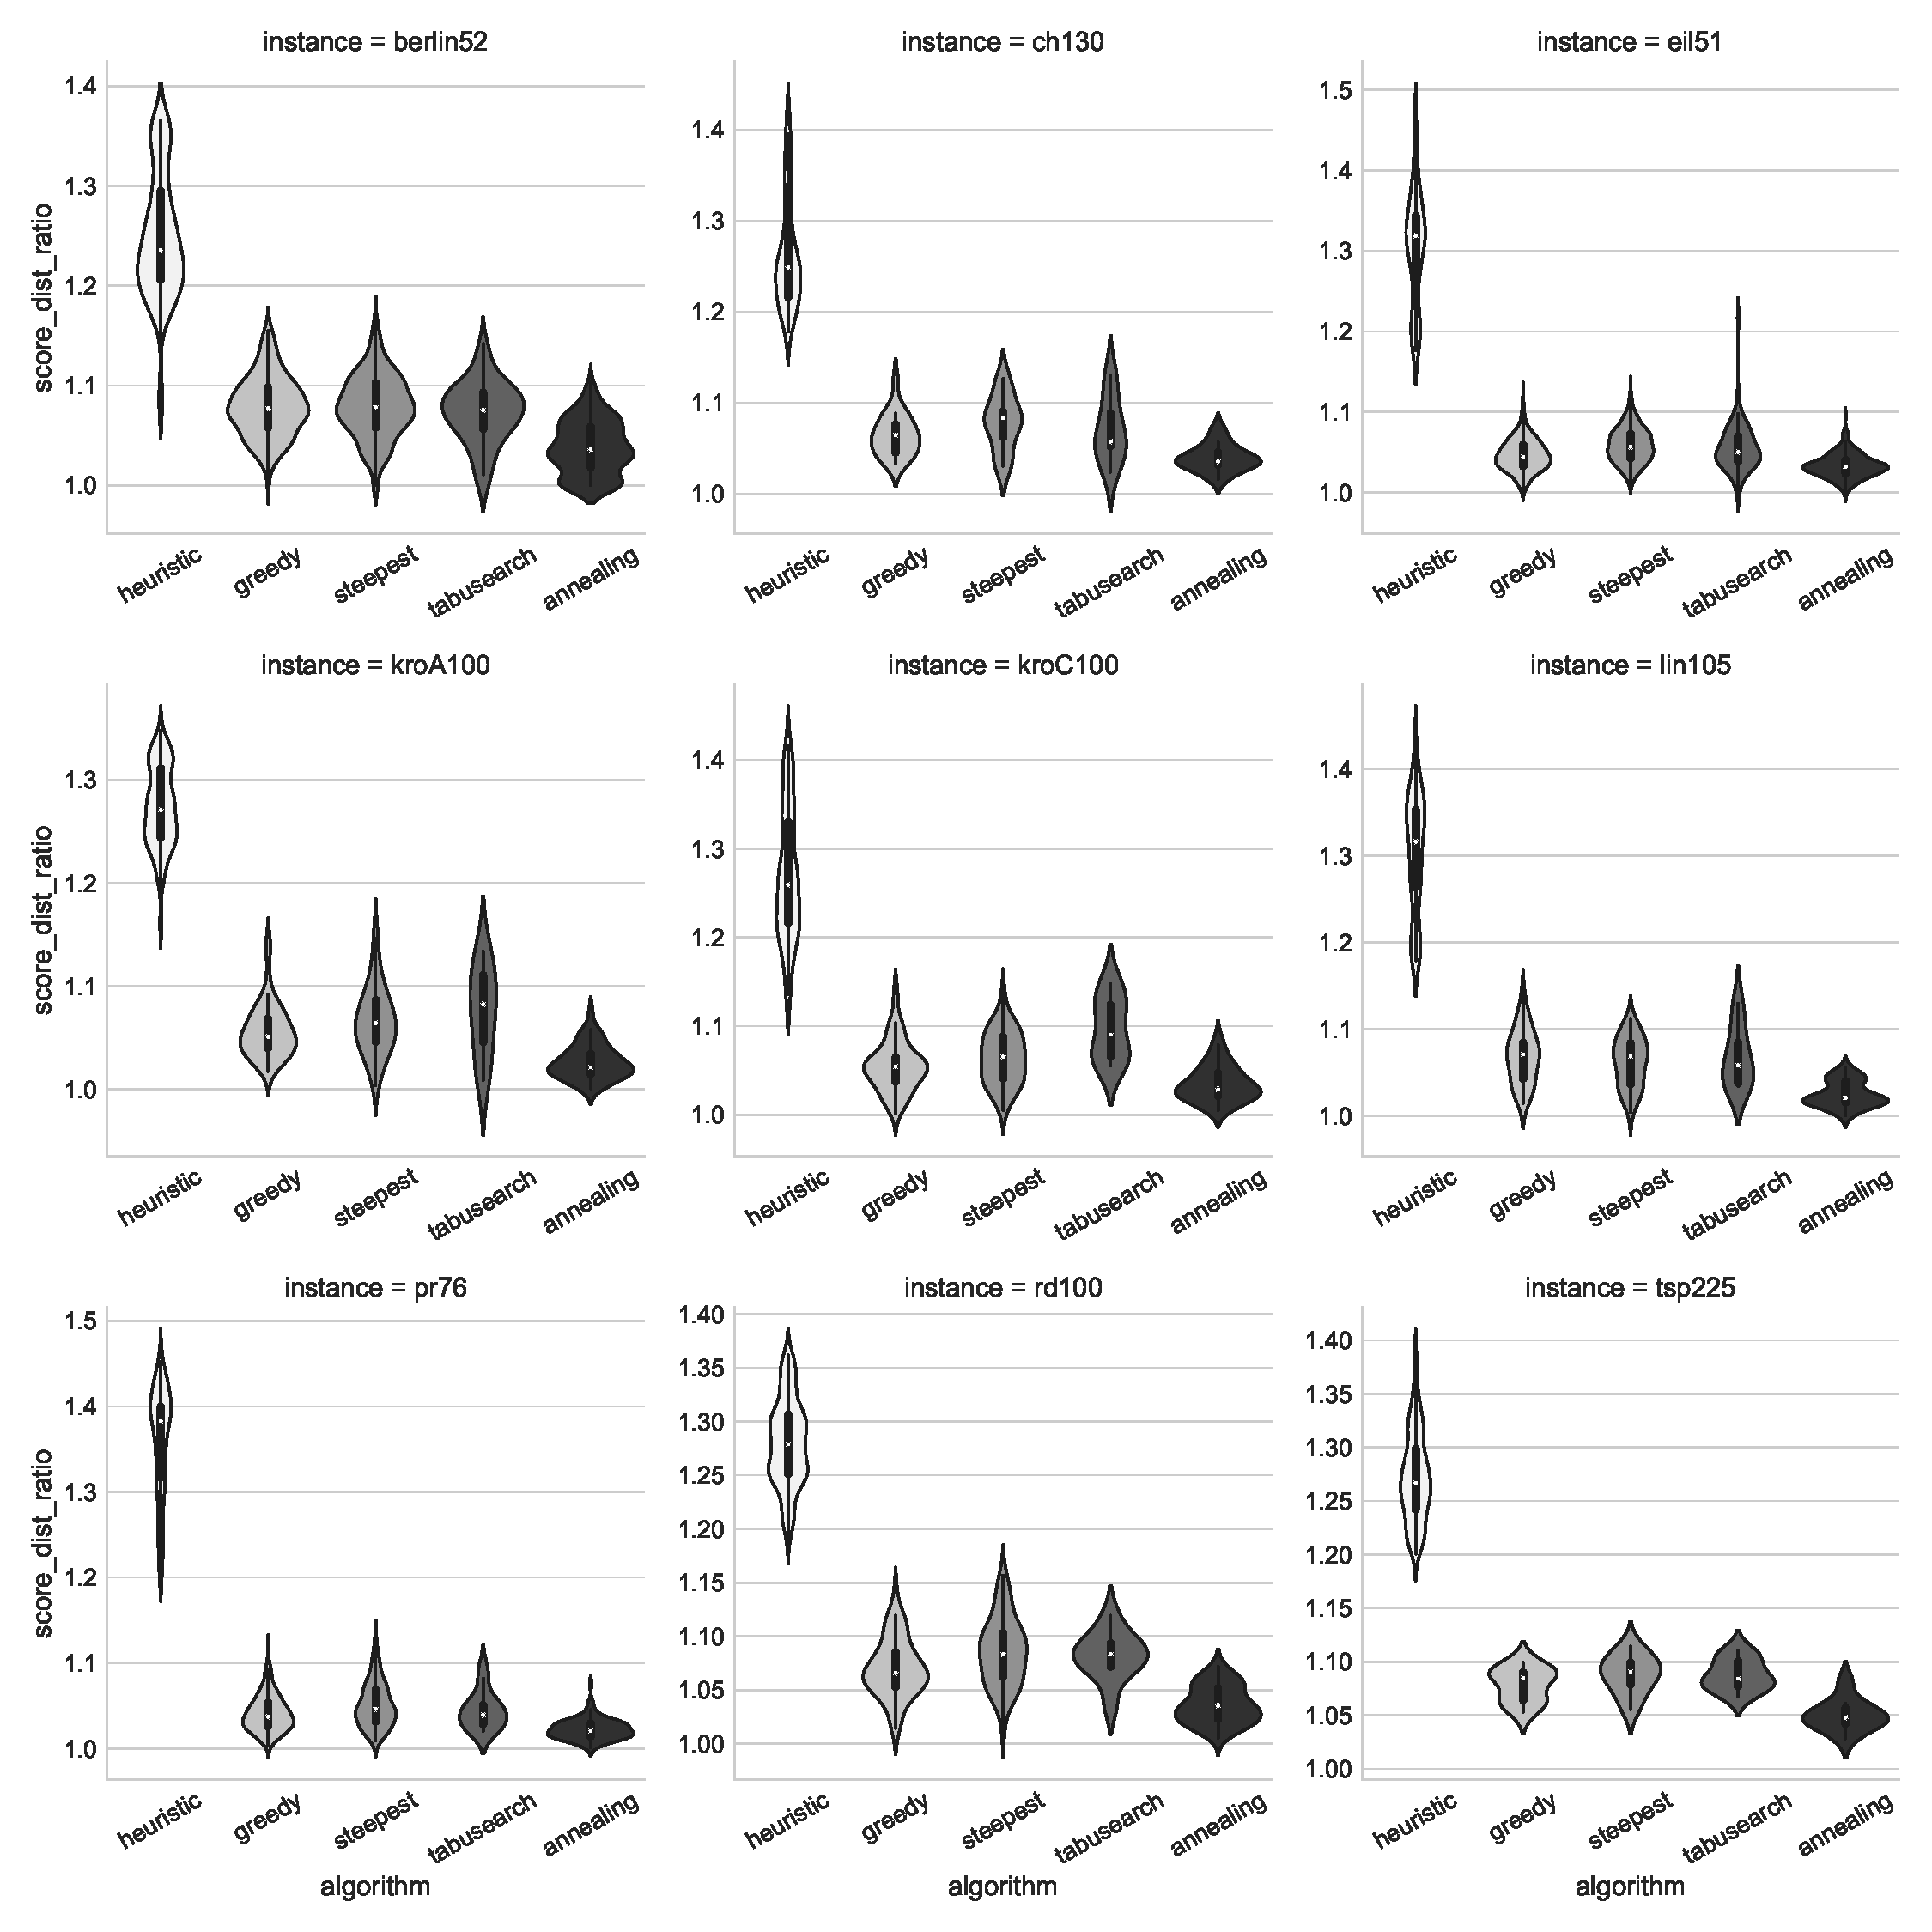
\includegraphics[width=1.0\textwidth]{graphs/score_comparison_violin.pdf}
\end{center}
\caption{Porównanie rozkładów znalezionych rozwiązań przez~algorytmy na~różnych instancjach.}
\label{fig:distribution}
\end{figure}

\subsection{Czas działania}

Algorytm losowy jest~zdecydowanie najszybszy, ponieważ sprawdza tylko jedno rozwiązanie. Podobnie heurystyka, jednak wyznaczenie przez nią~rozwiązania zajmuje trochę więcej czasu. Greedy i~Steepest przeszukują przestrzeń rozwiązań, dopóki nie~mogą już~bardziej poprawić wyniku, przez co~trwają zdecydowanie najdłużej. Przeważnie obliczenia Steepesta zajmują więcej czasu, niż~wykonanie algorytmu Greedy. Na~rys.~\ref{fig:time} można~też~zauważyć, że~pojedyncze wykonania trwają znacznie dłużej od~pozostałych --- szczególnie jest~to~widoczne przy~instancji berlin52.

\begin{figure}
\begin{center}
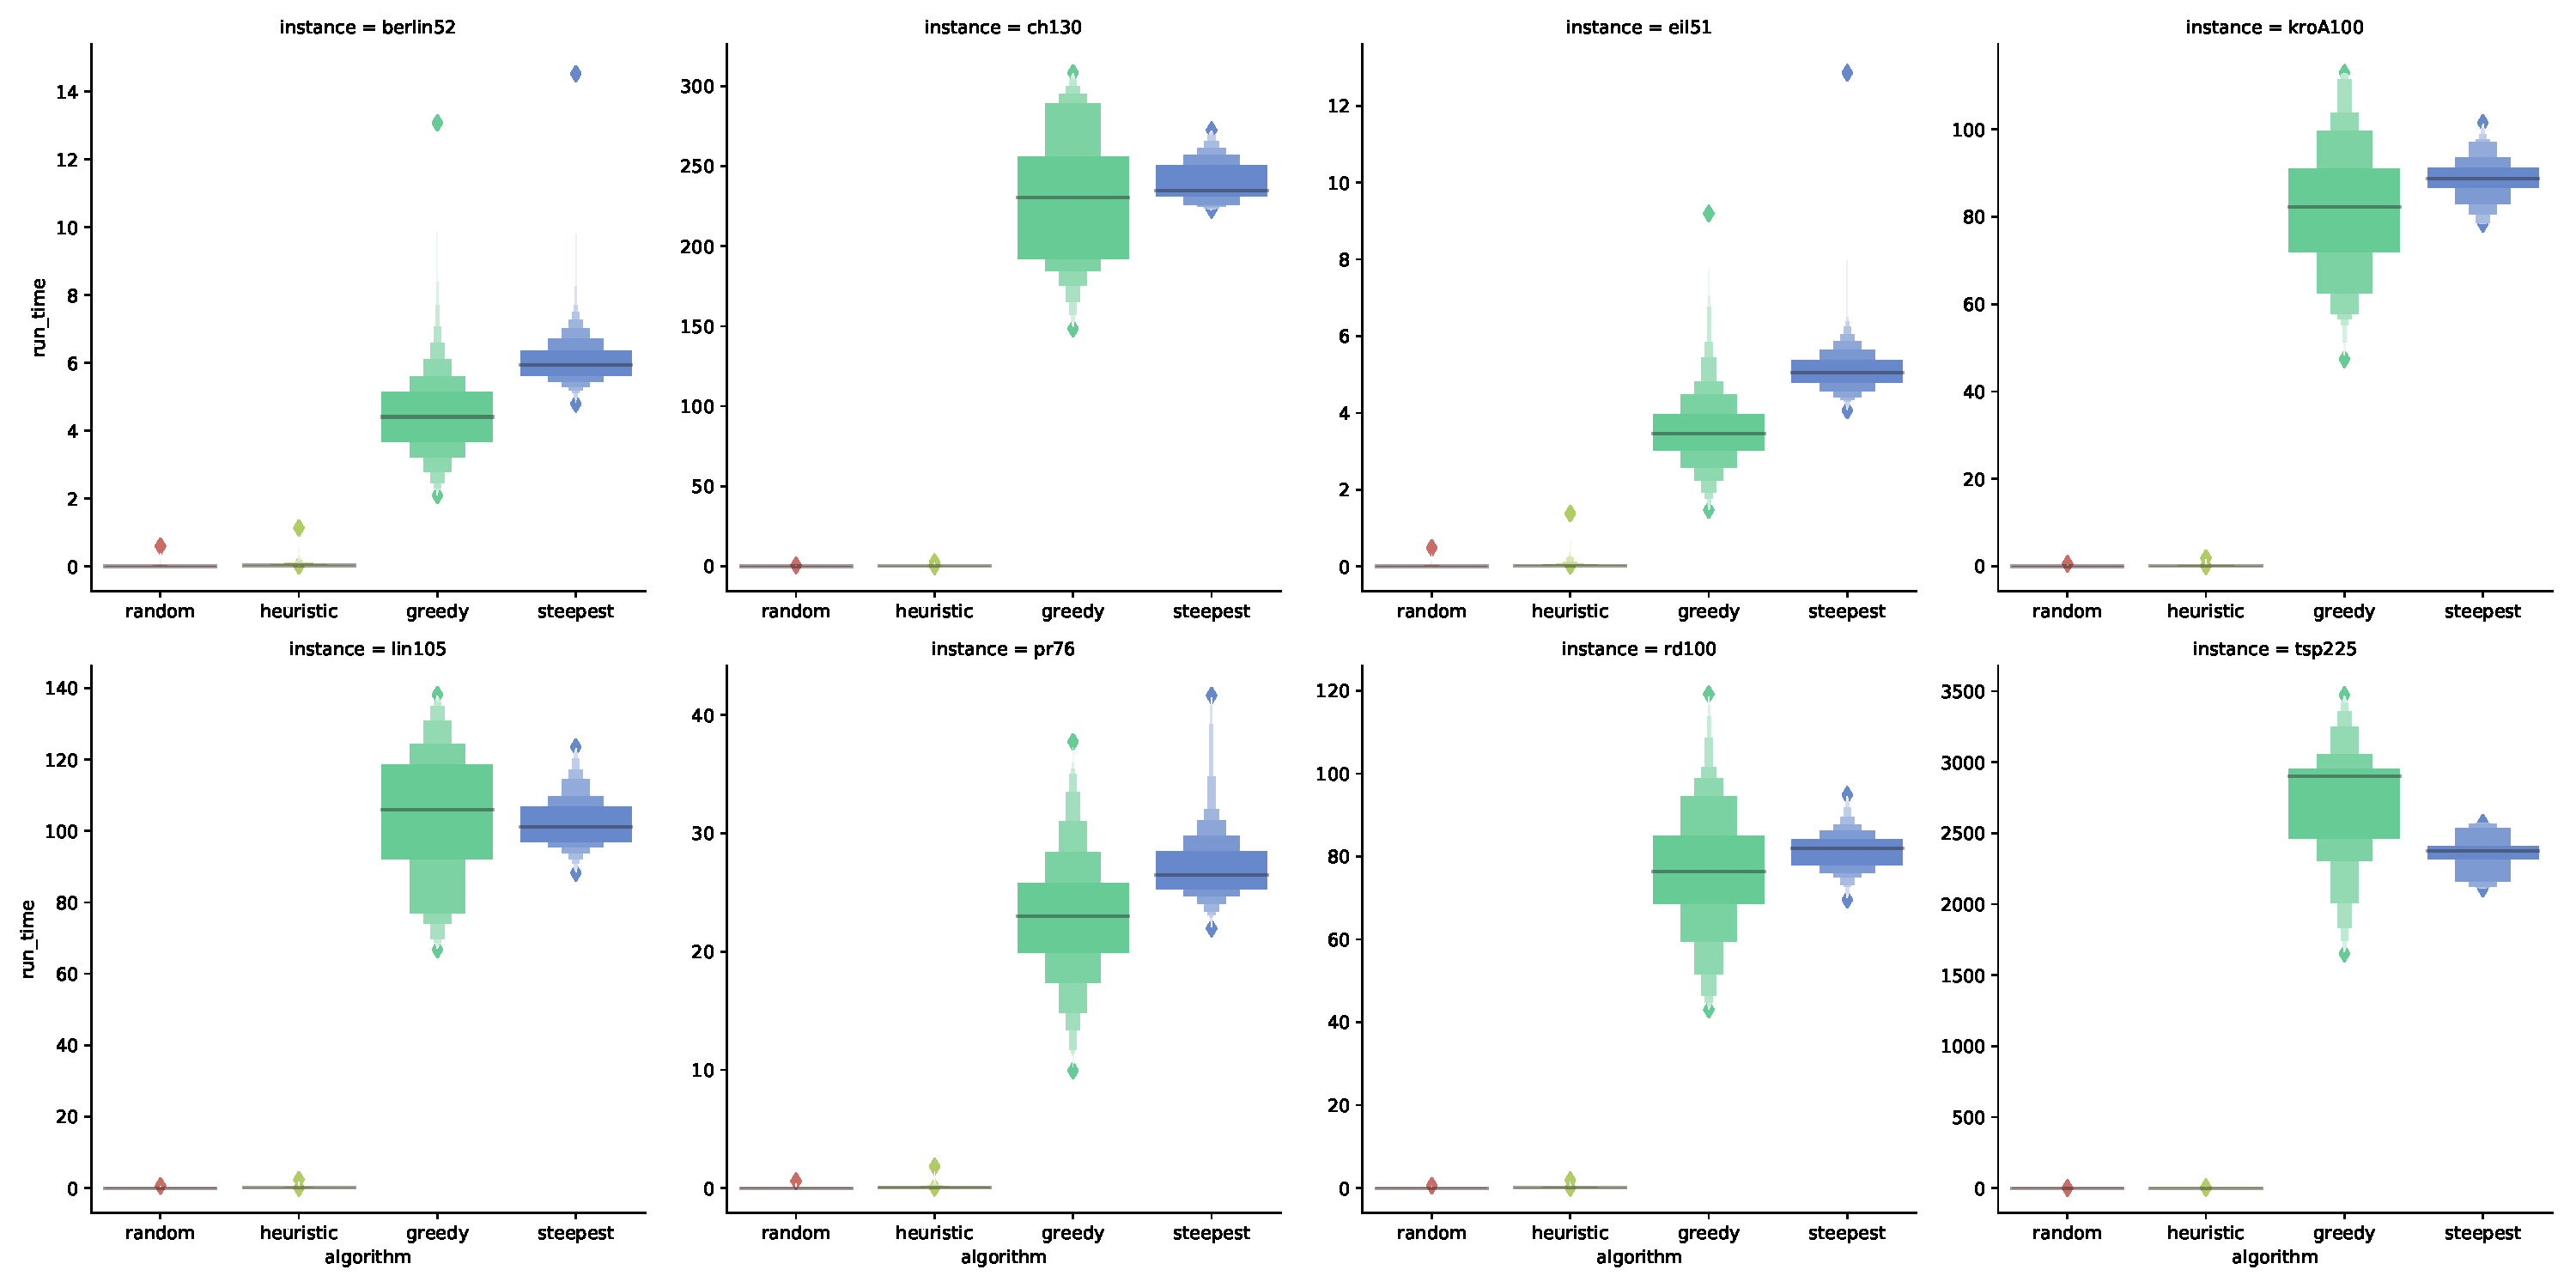
\includegraphics[width=1.0\textwidth]{graphs/time_comparison_letval.pdf}
\end{center}
\caption{Porównanie czasu działania algorytmów na~poszczególnych instancjach.}
\label{fig:time}
\end{figure}

\subsection{Efektywność algorytmów}

\subsubsection{Wybrana miara}

Aby porównać algorytmy pod~względem jakości, można to~zrobić przez zdefiniowanie kosztu czasowego, jaki~trzeba ponieść, aby~uzyskać dane rozwiązanie. Czyli należy policzyć iloraz $cost = time / result$, co~jest~przedstawione na~rys.~\ref{fig:cost}. Natomiast efektywnością algorytmu jest~odwrotność kosztu, która została przedstawiona na~rys.~\ref{fig:quality}.

\subsubsection{Wyniki}

Z~wykresów~\ref{fig:cost} i~\ref{fig:quality} można by~wyciągnąć wniosek, że~najefektywniejszym algorytmem jest~algorytm losowy, ponieważ zajmuje najmniej czasu. Takie wyniki są~jednak konsekwencją tego, że~przy każdy krok algorytmu przeszukiwania lokalnego jest~dość kosztowny, ponieważ przegląda się wiele rozwiązań, a~rozwiązanie jest~poprawiane nieznacznie (zgodnie z~założeniem algorytmów przeszukiwania lokalnego, że~funkcja celu sąsiadów niewiele się różni). Podobnie przy heurystyce --- nawet złożoność $\theta(n^2)$ nie~gwarantuje ulepszenia rozwiązania n-krotnie, a~jedynie kilkukrotnie, więc~koszt algorytmu jest~stosunkowo wysoki.

Na~wykresie kosztu widać również, że~Greedy jest~kosztowniejszy od~Steepesta, ponieważ daje zbliżone rozwiązania w~dłuższym czasie.

\begin{figure}
\begin{center}
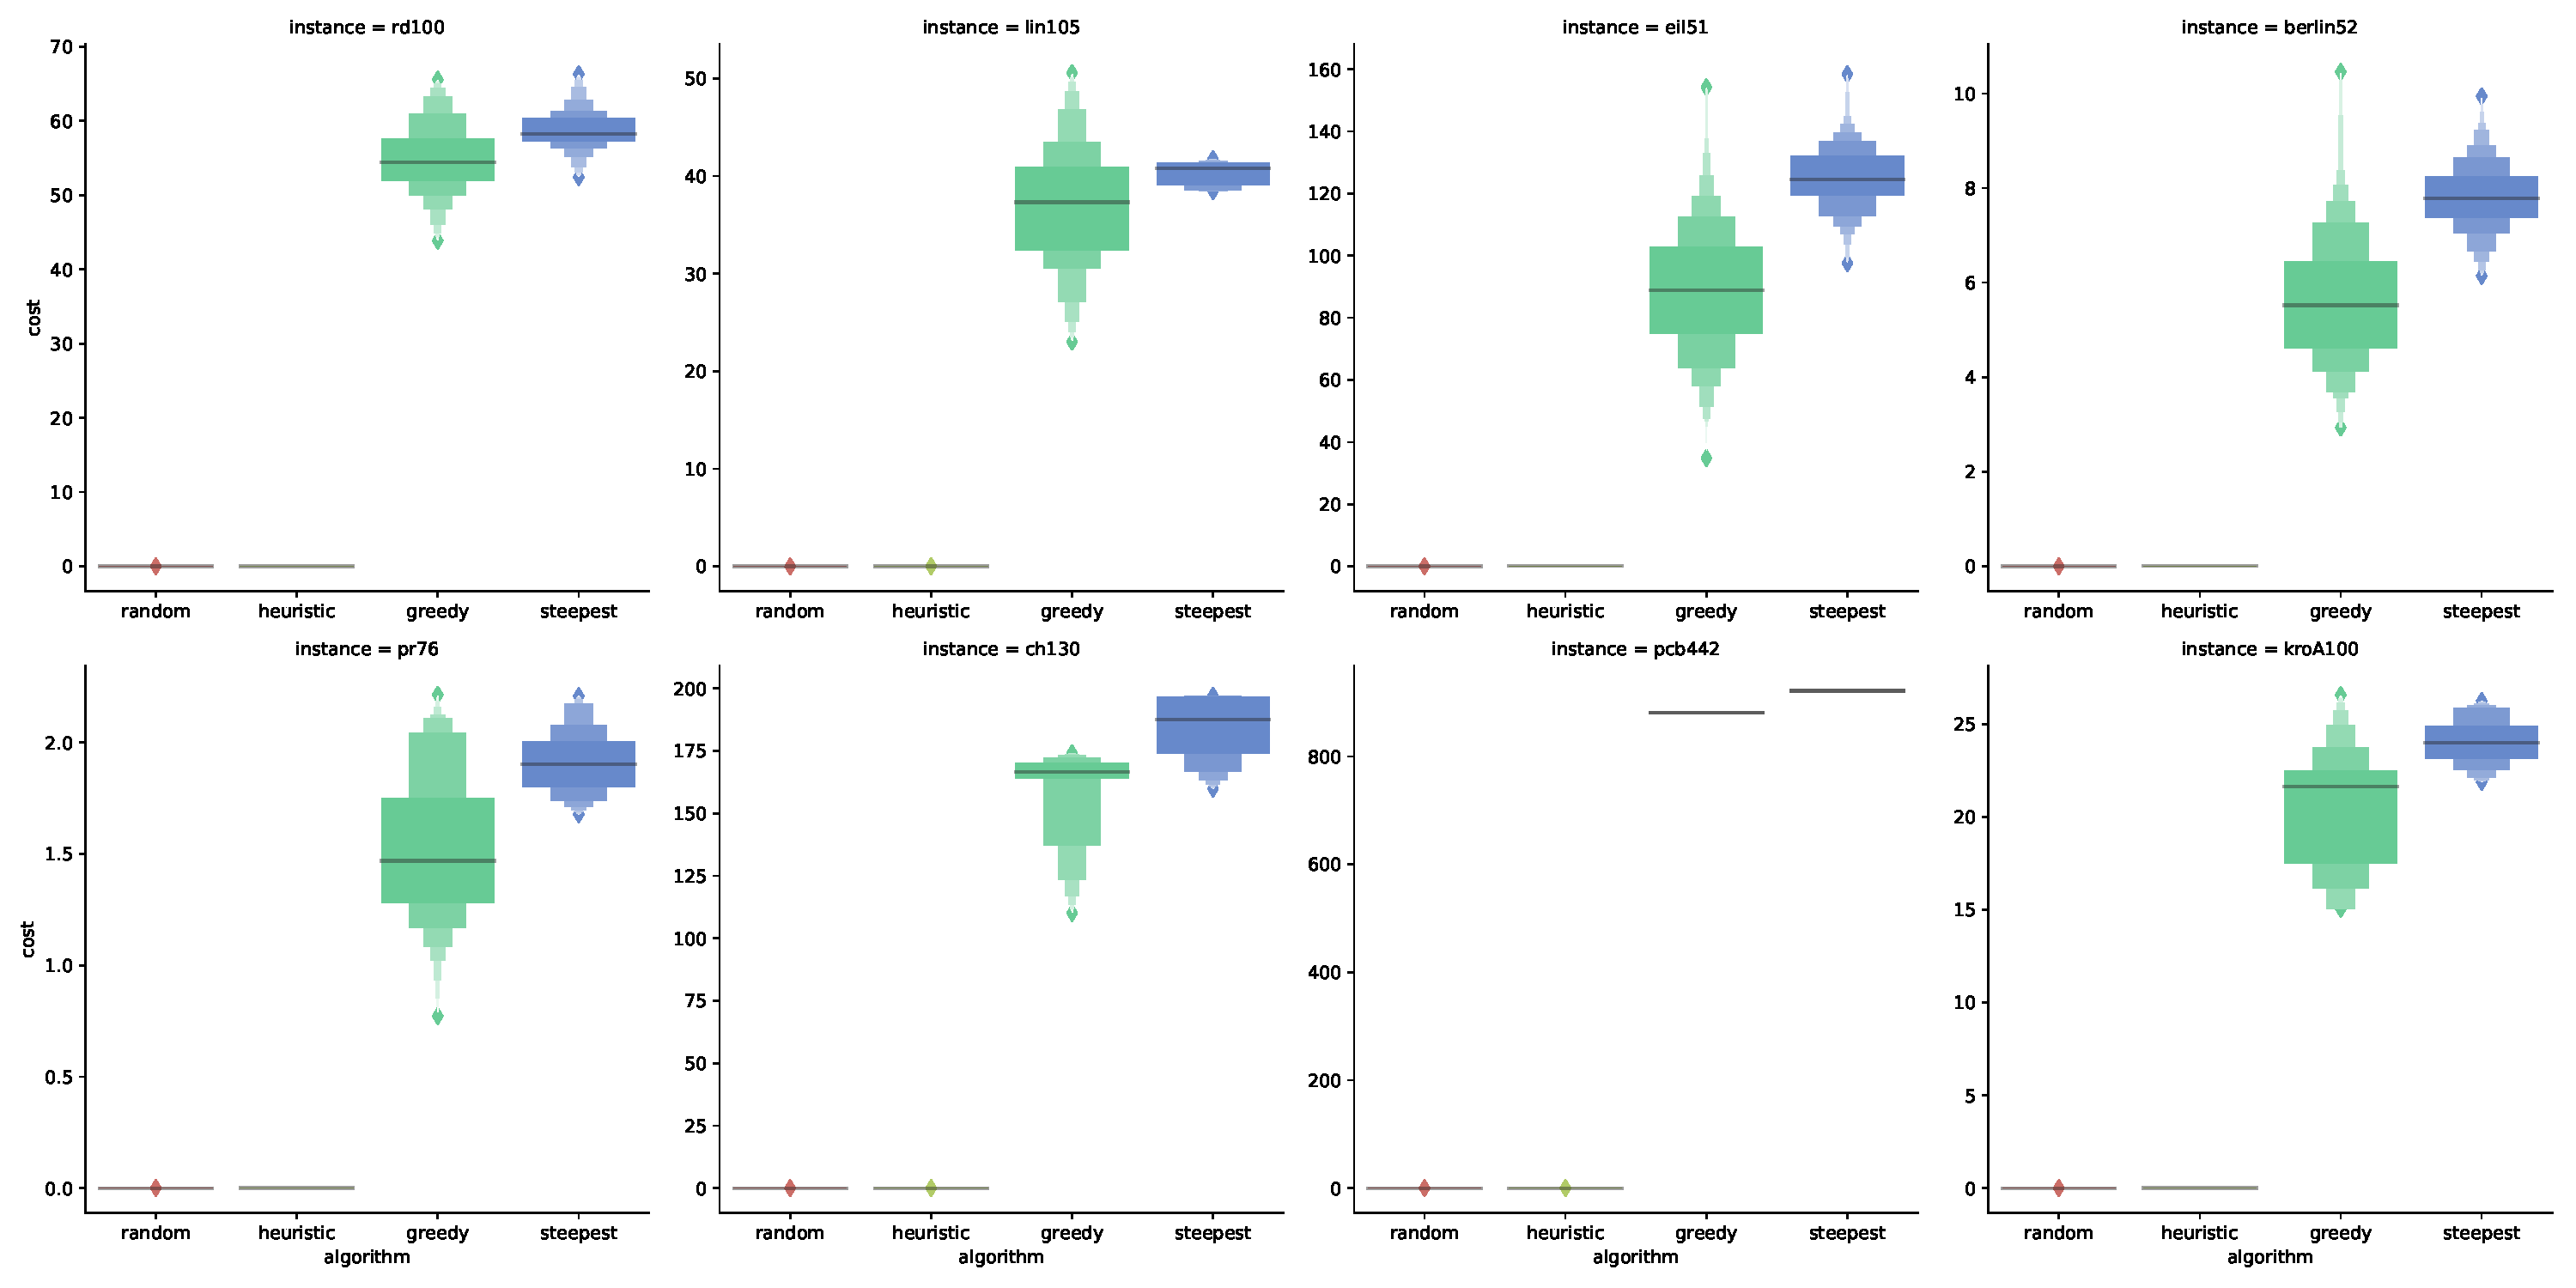
\includegraphics[width=1.0\textwidth]{graphs/cost_comparison_letval.pdf}
\end{center}
\caption{Porównanie kosztów algorytmów na~poszczególnych instancjach.}
\label{fig:cost}
\end{figure}

\begin{figure}
\begin{center}
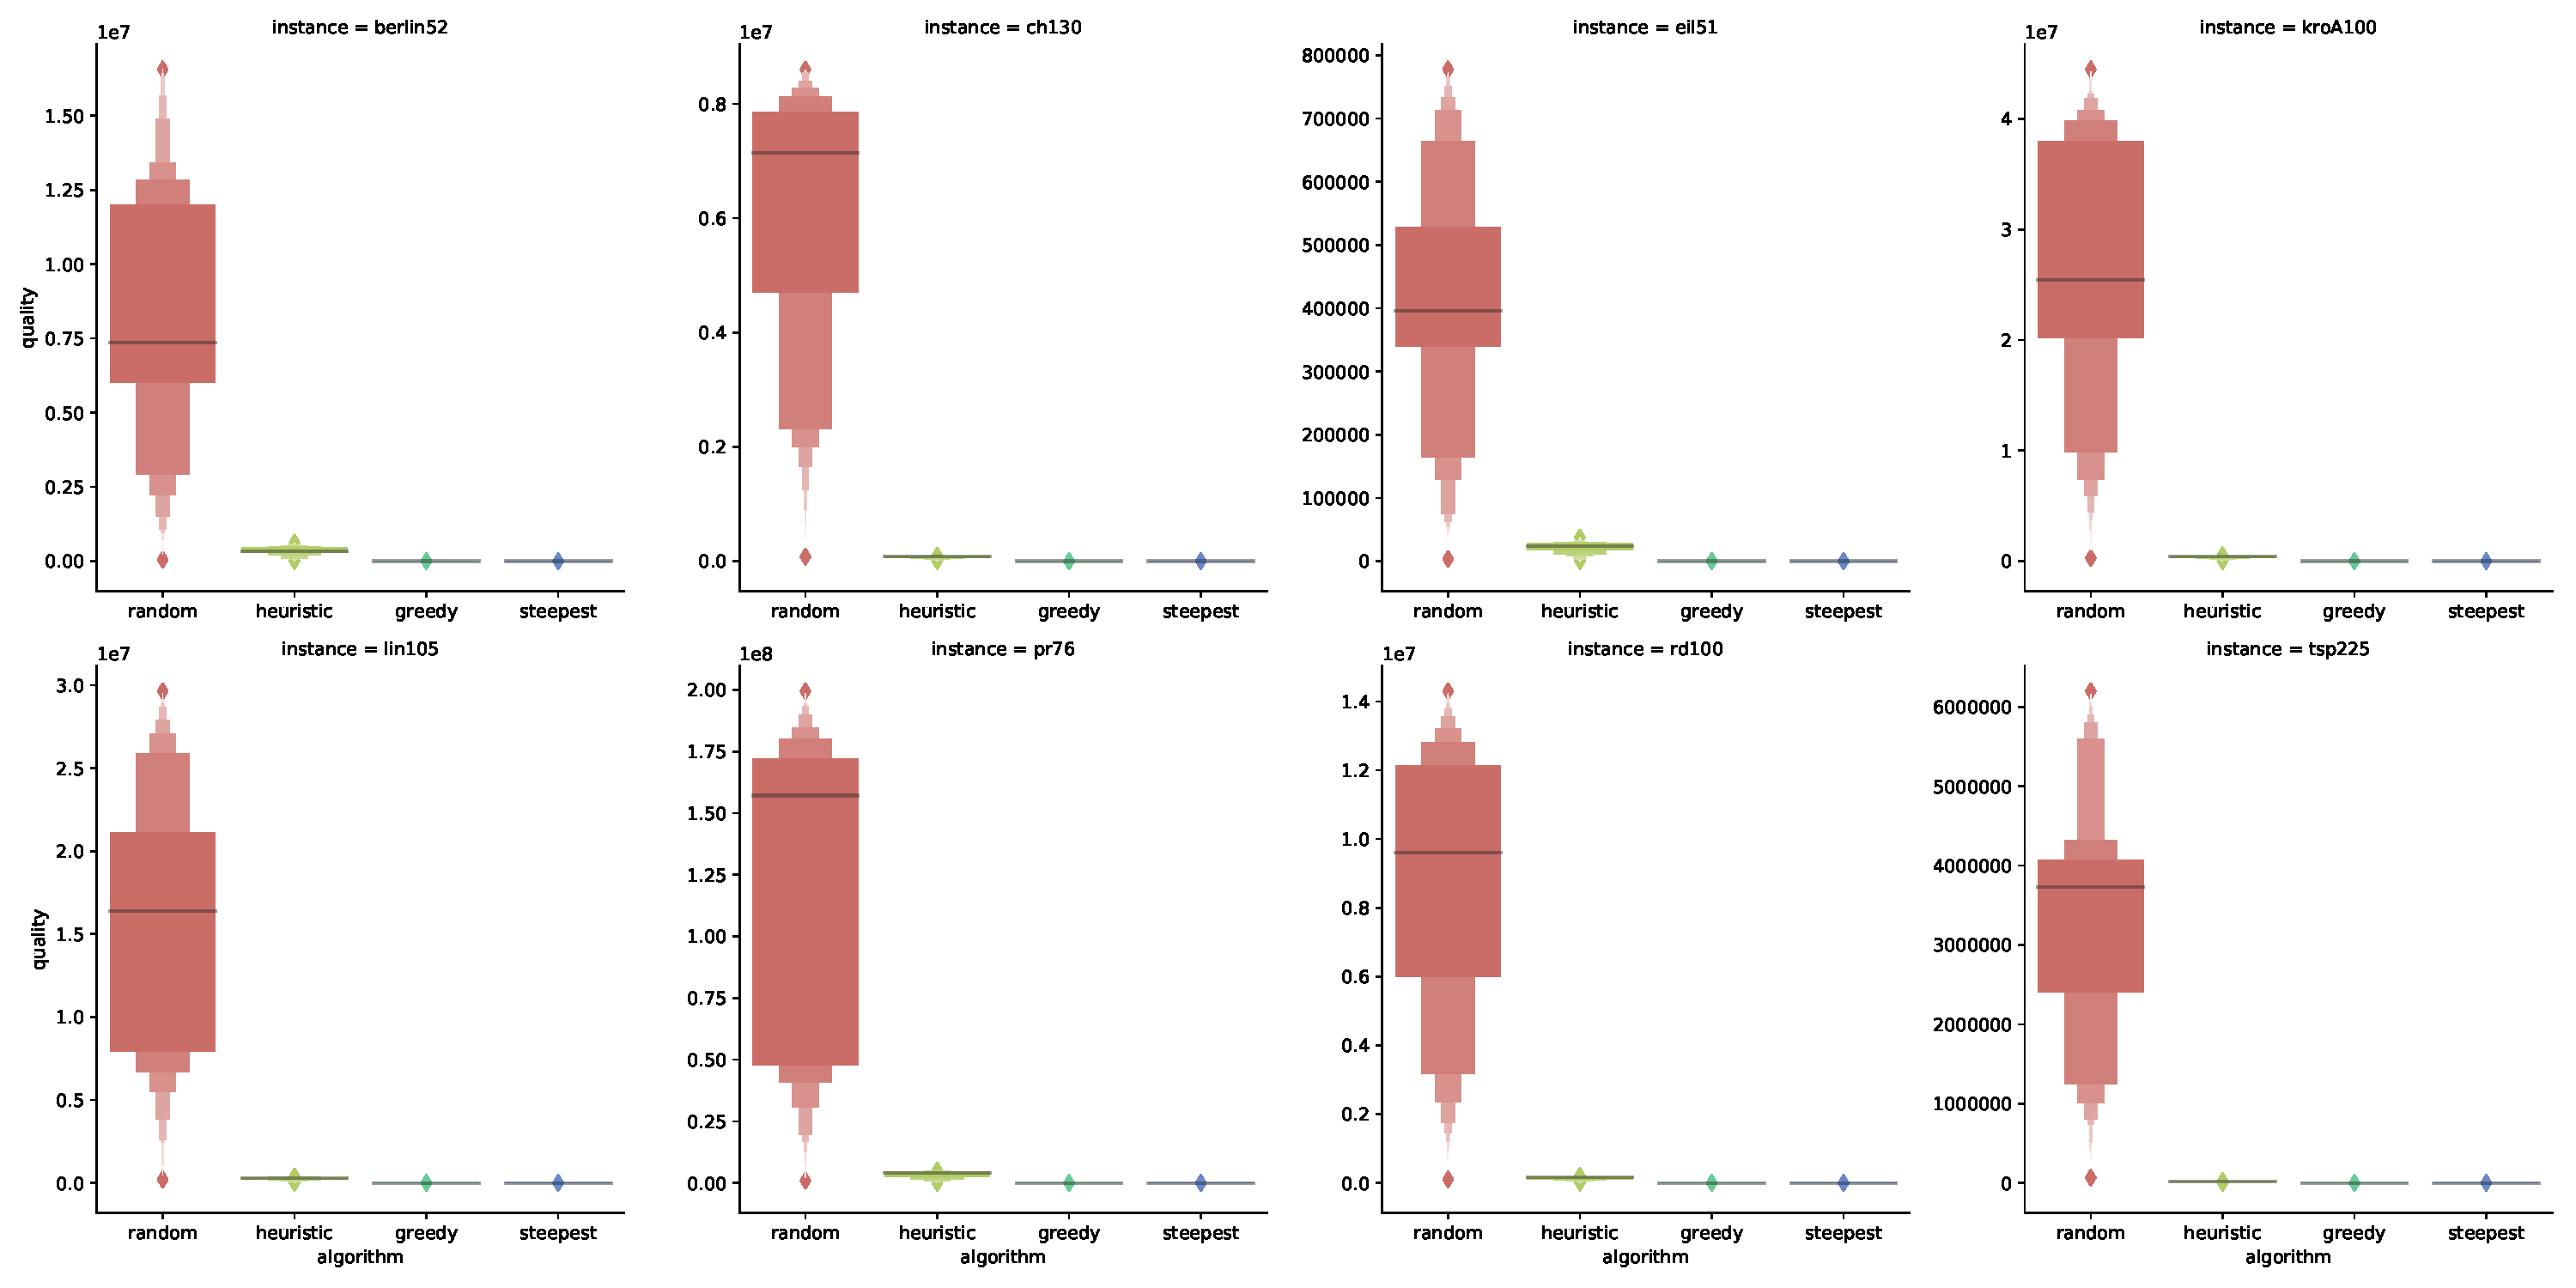
\includegraphics[width=1.0\textwidth]{graphs/quality_comparison_letval.pdf}
\end{center}
\caption{Porównanie efektywności algorytmów na~poszczególnych instancjach.}
\label{fig:quality}
\end{figure}

\subsection{Liczba kroków algorytmów lokalnego przeszukiwania}

Wykres~\ref{fig:steps} przedstawia liczbę kroków wykonanych przez algorytmy lokalnego przeszukiwania. Widać, że~Greedy wykonuje ich kilkakrotnie więcej niż~Steepest, a~także, że~liczba wykonanych kroków przez ten~algorytm jest~dużo bardziej zróżnicowana, w~zależności od~przypadku startowego. Jest~to~spowodowane tym, że~algorytm Steepest we~wcześniejszym kroku osiąga lokalnie najlepsze rozwiązanie, ponieważ za~każdym razem wybiera to, które~najbardziej poprawia wynik z~całego sąsiedztwa.

\begin{figure}
\begin{center}
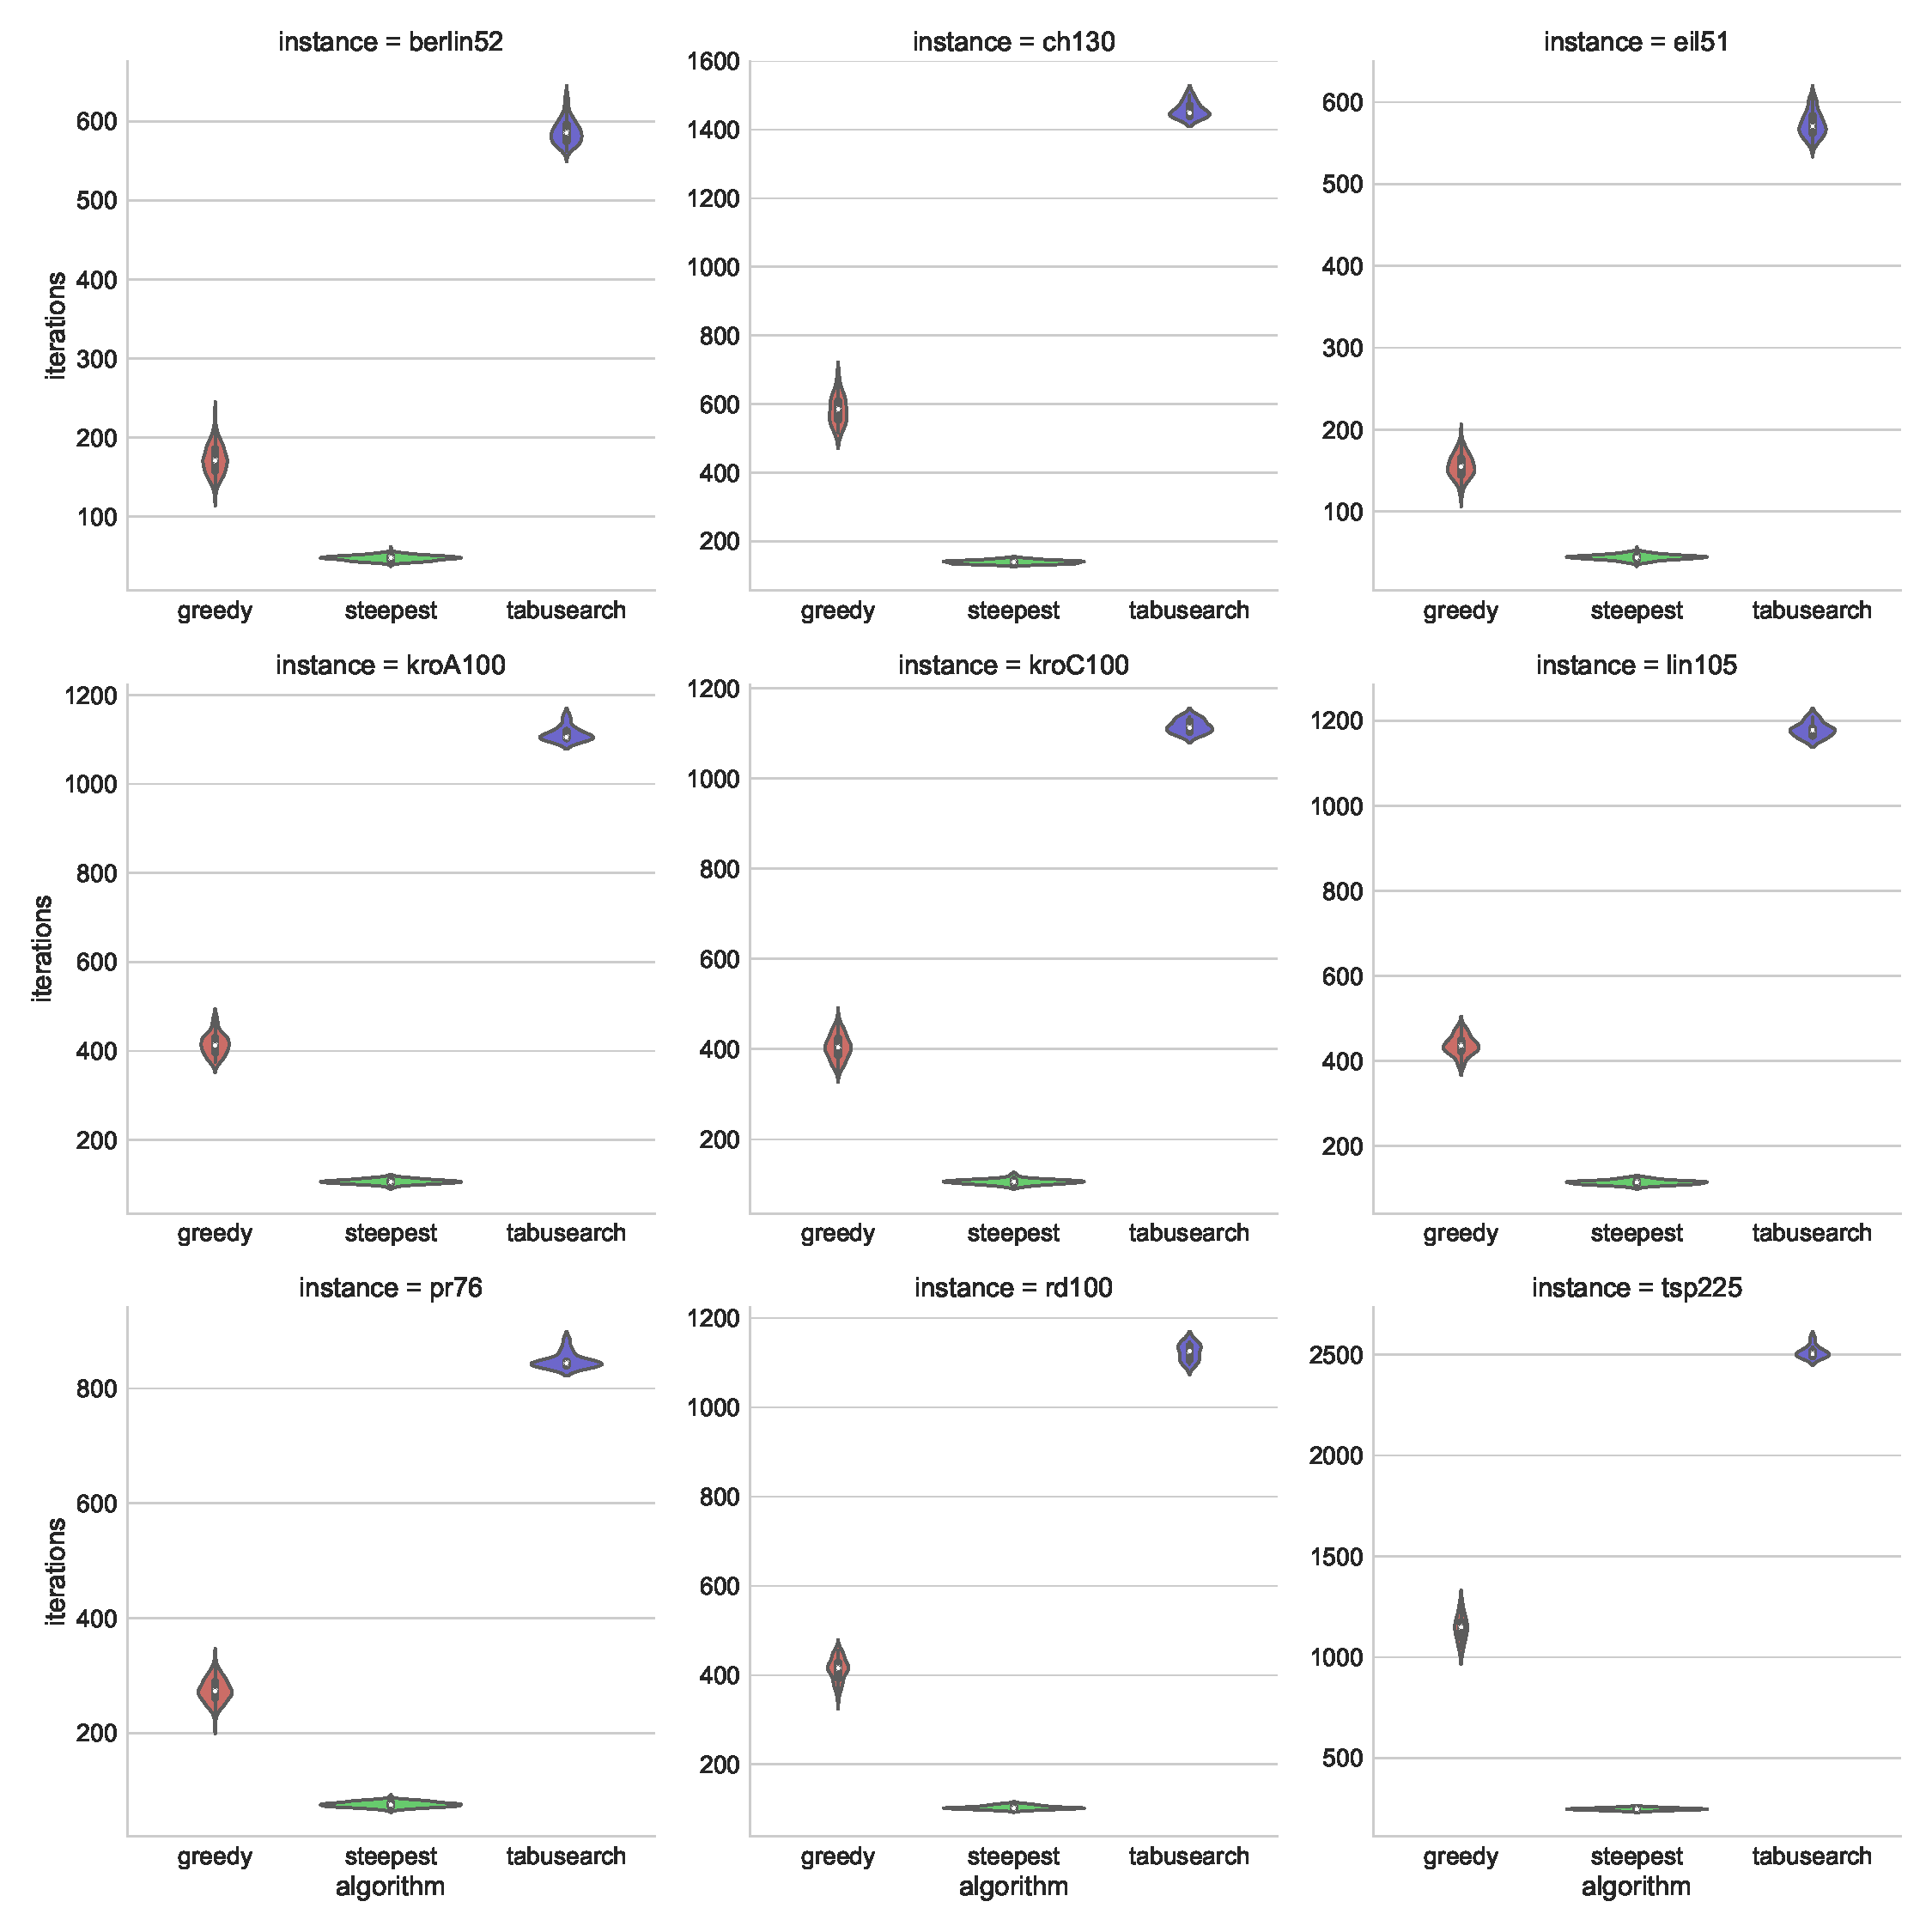
\includegraphics[width=1.0\textwidth]{graphs/iterations_comparison_violin.pdf}
\end{center}
\caption{Porównanie algorytmów Greedy Search i~Steepest pod~względem liczby kroków do~zatrzymania.}
\label{fig:steps}
\end{figure}

\subsection{Średnia liczba przeszukanych rozwiązań}

Na~wykresie \ref{fig:nsol} jest~przedstawiona liczba rozwiązań przeszukiwanych przez~oba rozważane algorytmy lokalnego przeszukiwania. Można na~nim~zauważyć, że~średnio Steepest przeszukuje większą przestrzeń, choć~zdarzają się wykonania algorytmu Greedy, które~sprawdzają większą liczbę rozwiązań. Jest to~o~tyle ciekawe, że~Steepest wykonuje mniej kroków, niż~Greedy, a~i~tak aby~je~wykonać, przegląda więcej rozwiązań. Co~ciekawe, ta~tendencja jest~odmienna dla~największej instancji, podobnie~też, czas działania algorytmu Greedy dla~niej jest~większy od~Steepesta.

\begin{figure}
\begin{center}
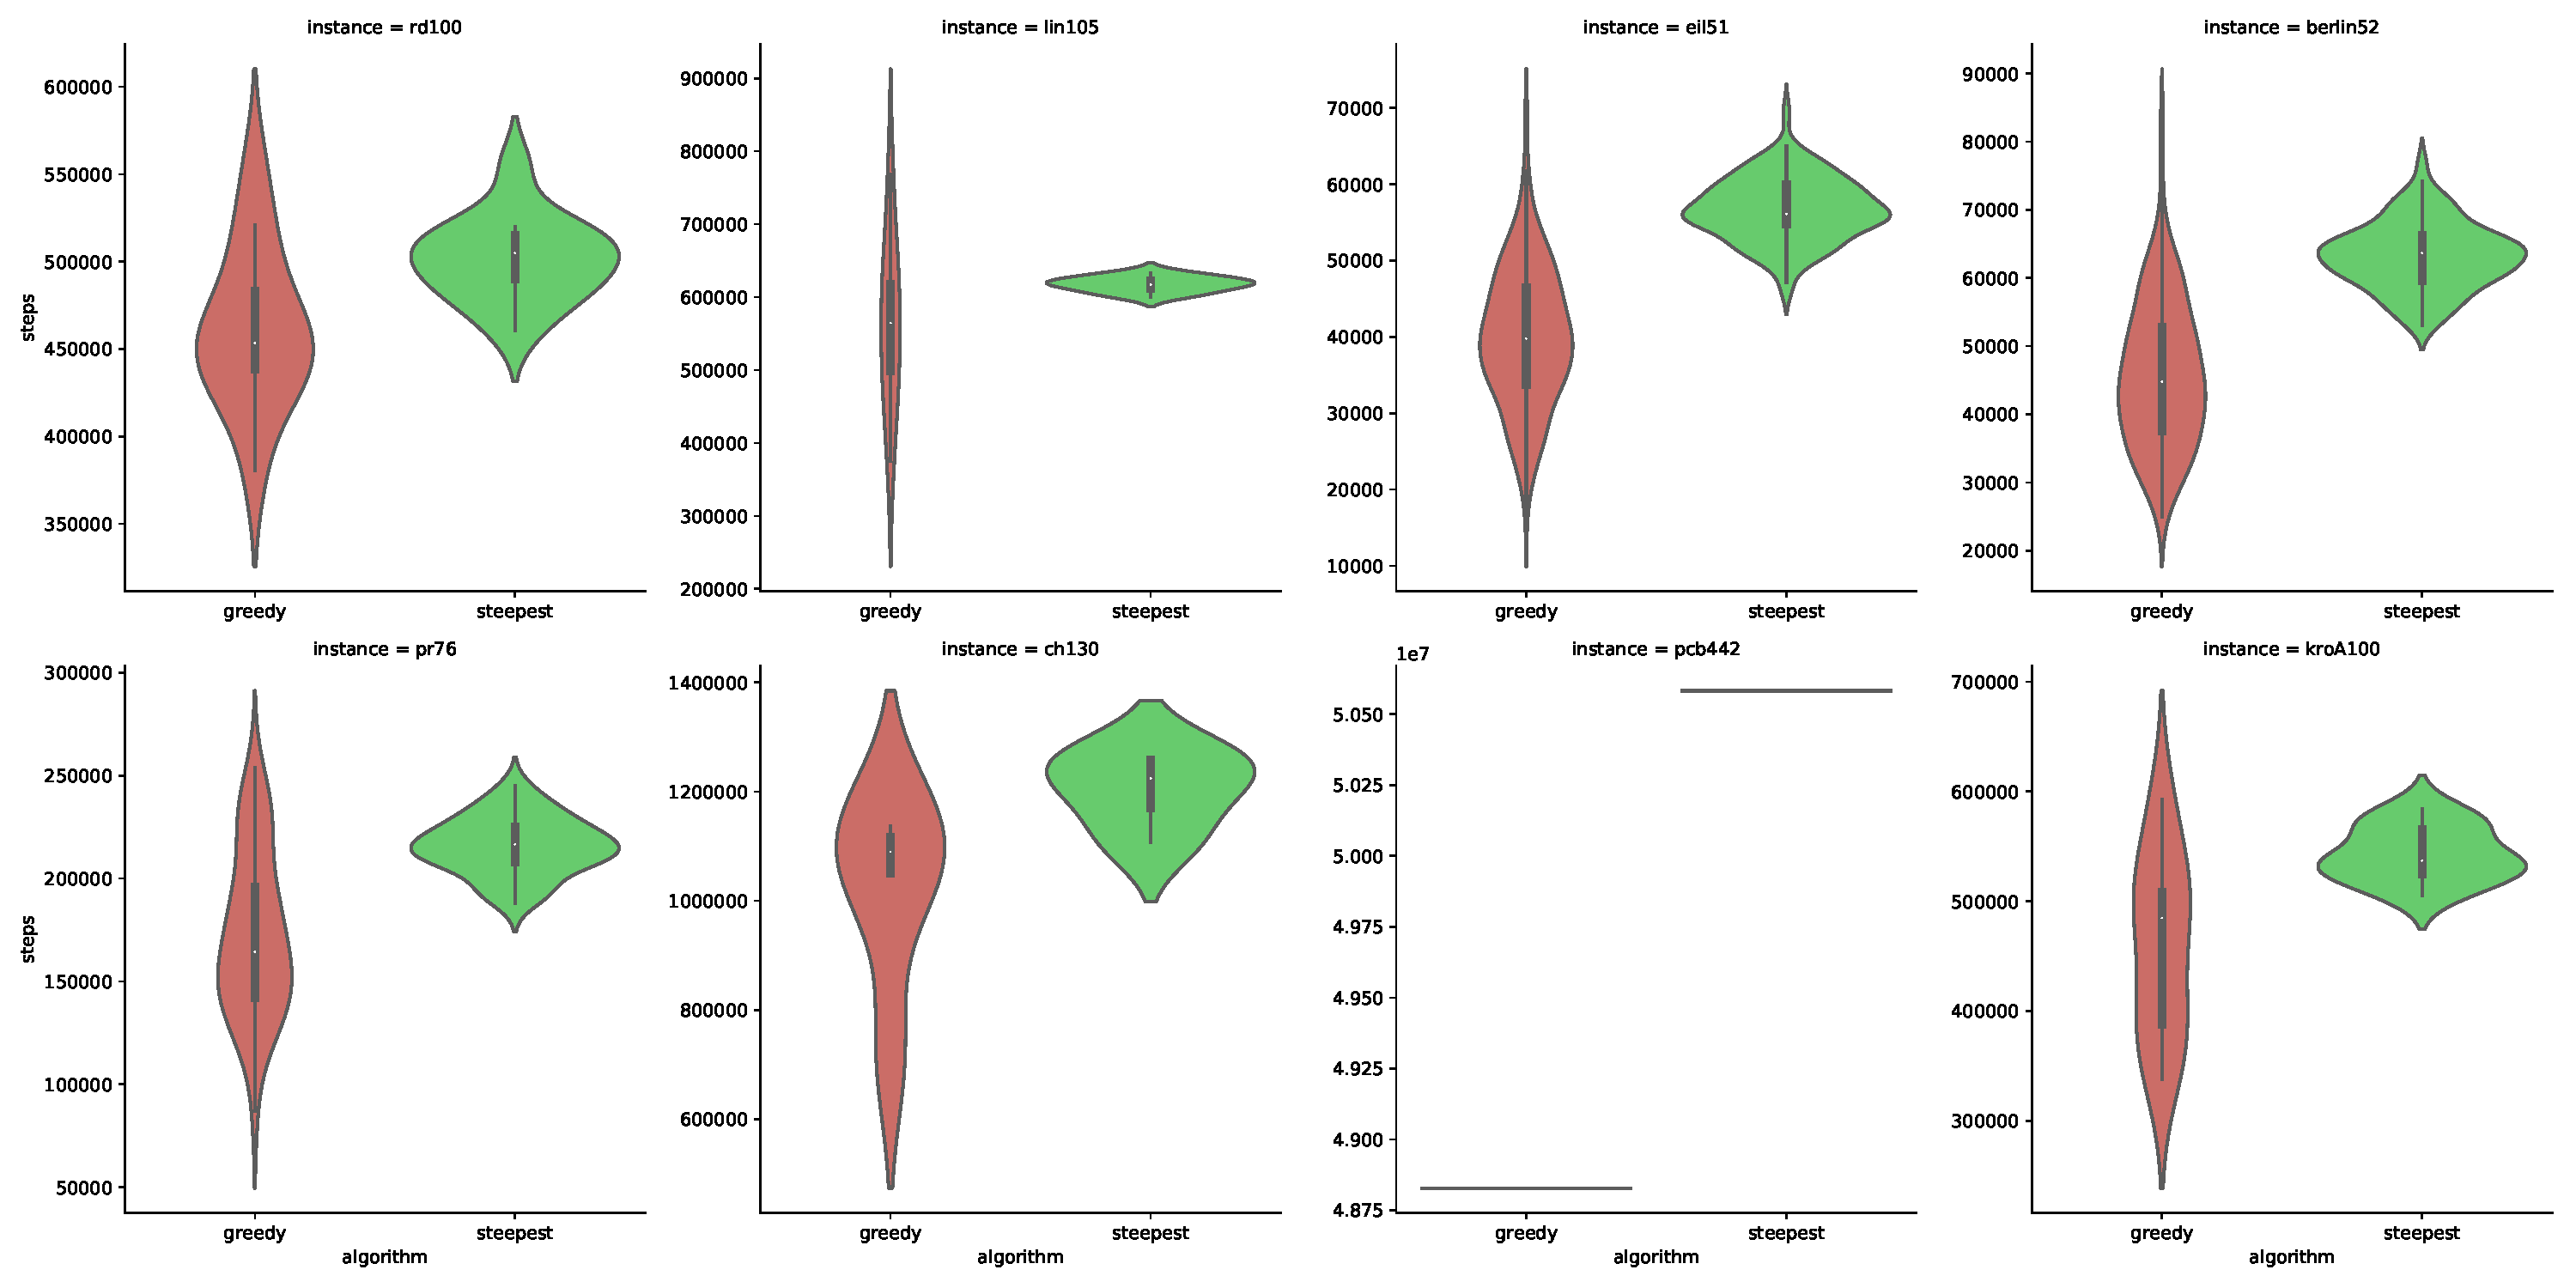
\includegraphics[width=1.0\textwidth]{graphs/steps_comparison_violin.pdf}
\end{center}
\caption{Porównanie algorytmów Greedy Search i~Steepest pod~względem liczby przeszukanych rozwiązań.}
\label{fig:nsol}
\end{figure}

\subsection{Przeszukiwanie lokalne}

\subsubsection{Jakość rozwiązania początkowego a końcowego}

Badając zależność między rozwiązaniem początkowym, a~końcowym, nie~udało nam się zaobserwować związku na~wykresie punktowym \ref{fig:diff_point}. Punkty są~bardzo rozrzucone i~nie~daje się ich~odpowiednio pogrupować. Na~wykresie skrzypcowym~\ref{fig:diff} zostały przedstawione rozwiązania początkowe i~końcowe dla~obu~algorytmów. Widać, że~są~wyraźnie od~siebie oddalone i~zgrupowane w~osobne chmury. Można zatem przypuszczać, że~jakość rozwiązania końcowego nie~zależy od~jakości rozwiązania początkowego.

\begin{figure}
\begin{center}
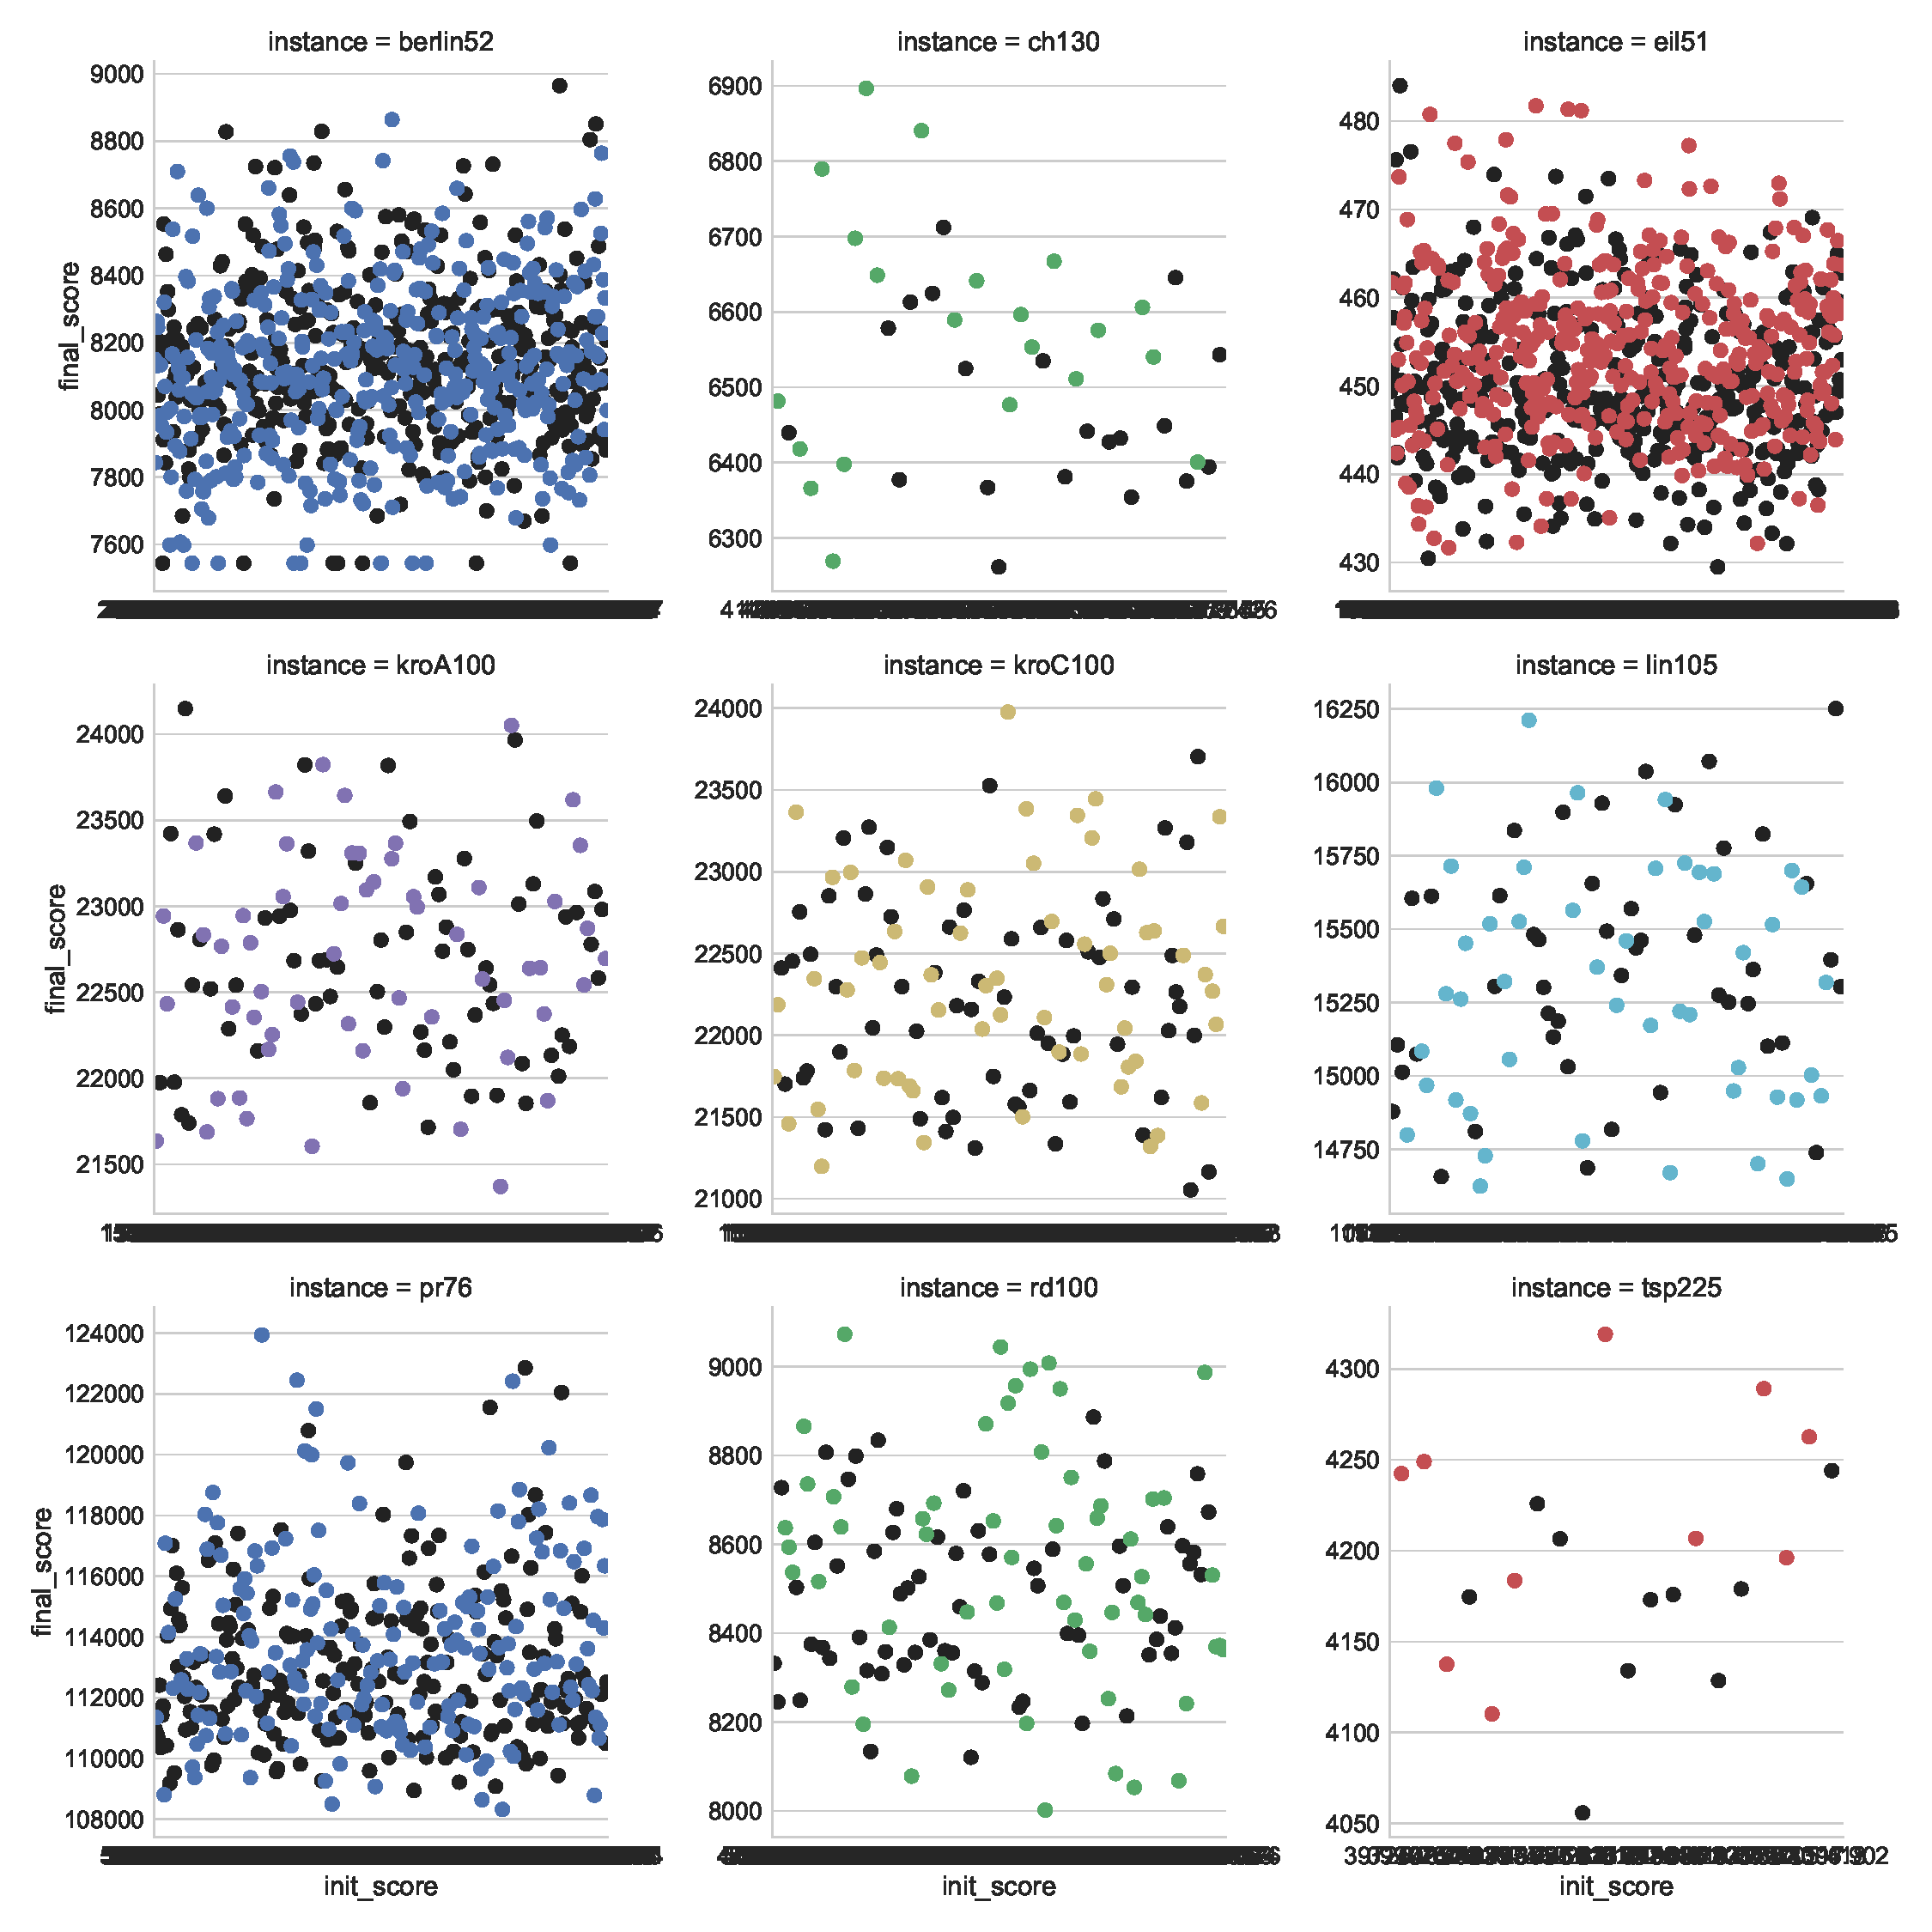
\includegraphics[width=1.0\textwidth]{graphs/init_vs_final_score_point.pdf}
\end{center}
\caption{Porównanie jakości rozwiązań początkowych i~końcowych przez~algorytmy Greedy Search i~Steepest przedstawione na wykresie punktowym.}
\label{fig:diff_point}
\end{figure}

\begin{figure}
\begin{center}
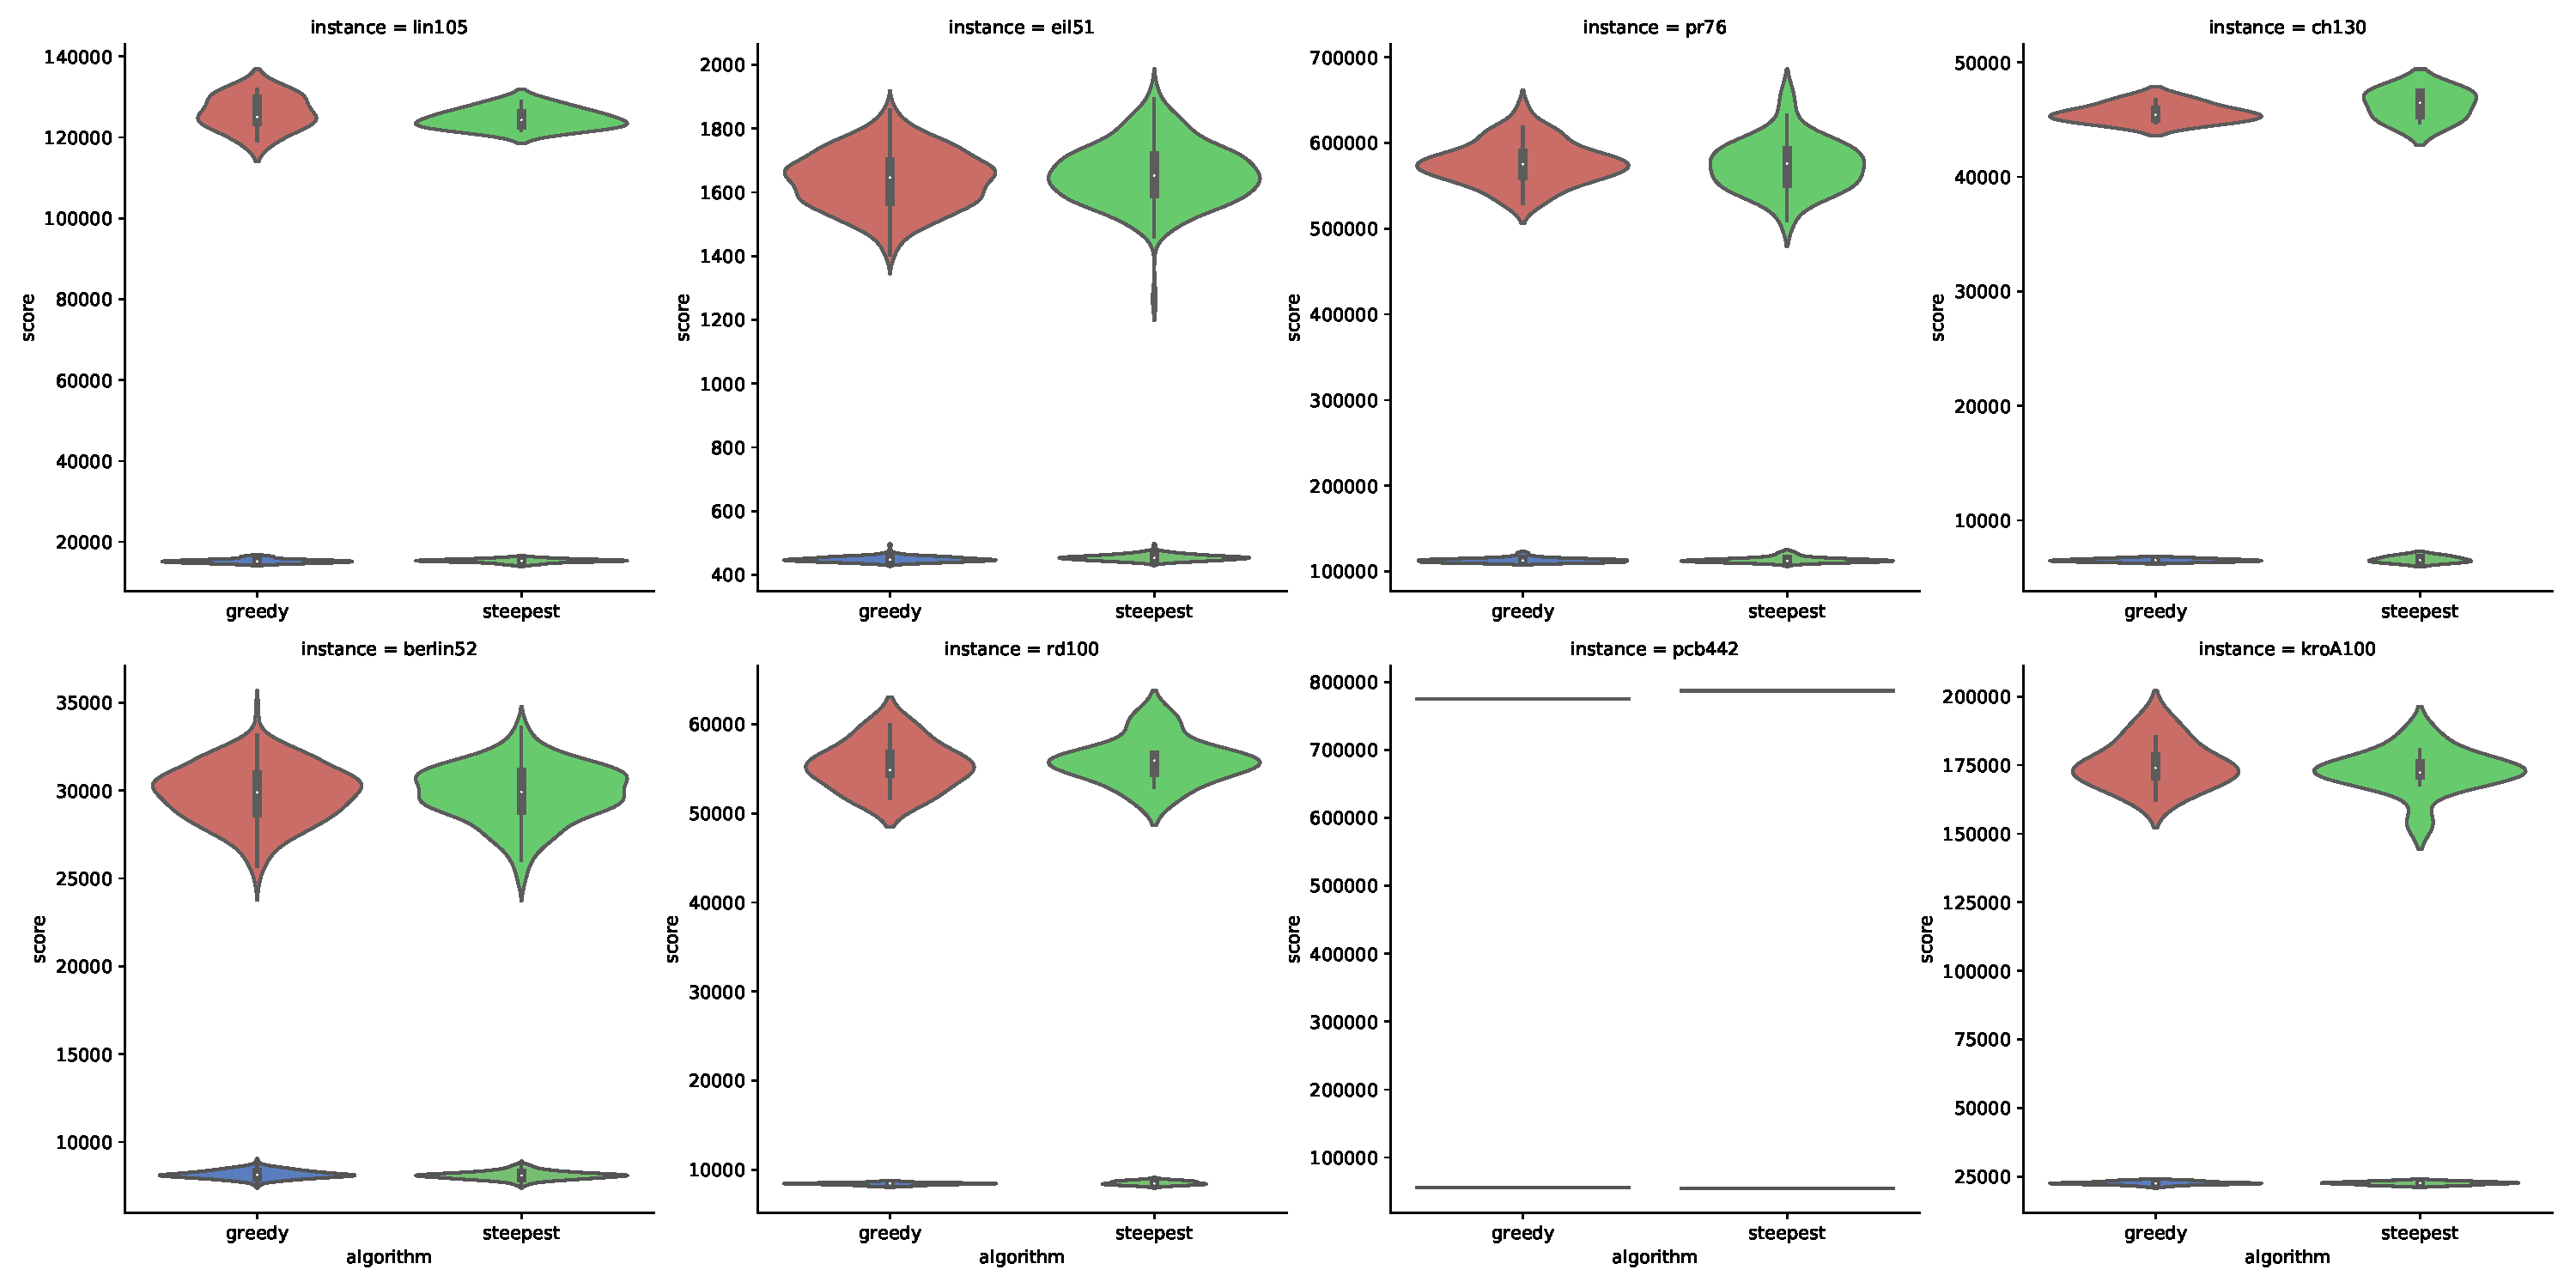
\includegraphics[width=1.0\textwidth]{graphs/init_vs_final_score_violin.pdf}
\end{center}
\caption{Porównanie jakości rozwiązań początkowych i~końcowych przez~algorytmy Greedy Search i~Steepest.}
\label{fig:diff}
\end{figure}

\subsubsection{Wielokrotne uruchamianie dla różnych rozwiązań początkowych}

Wykresy~\ref{fig:more_berlin} i~\ref{fig:more_eil} przedstawiają wartość najlepszego znalezionego rozwiązania po~i-tej iteracji. Jak~widać, poprawia się ona~co~pewien czas. Im~rozwiązanie jest lepsze, tym~ten~czas jest~dłuższy. Im~więcej razy algorytm będzie uruchamiany z~różnych rozwiązań początkowych, tym~istnieje większa szansa, że~osiągnie on~lepszy wynik, więc~warto powtarzać uruchomienia dla~różnych rozwiązań początkowych, aby~pełniej przeszukać przestrzeń wszystkich rozwiązań.

\begin{figure}
\begin{center}
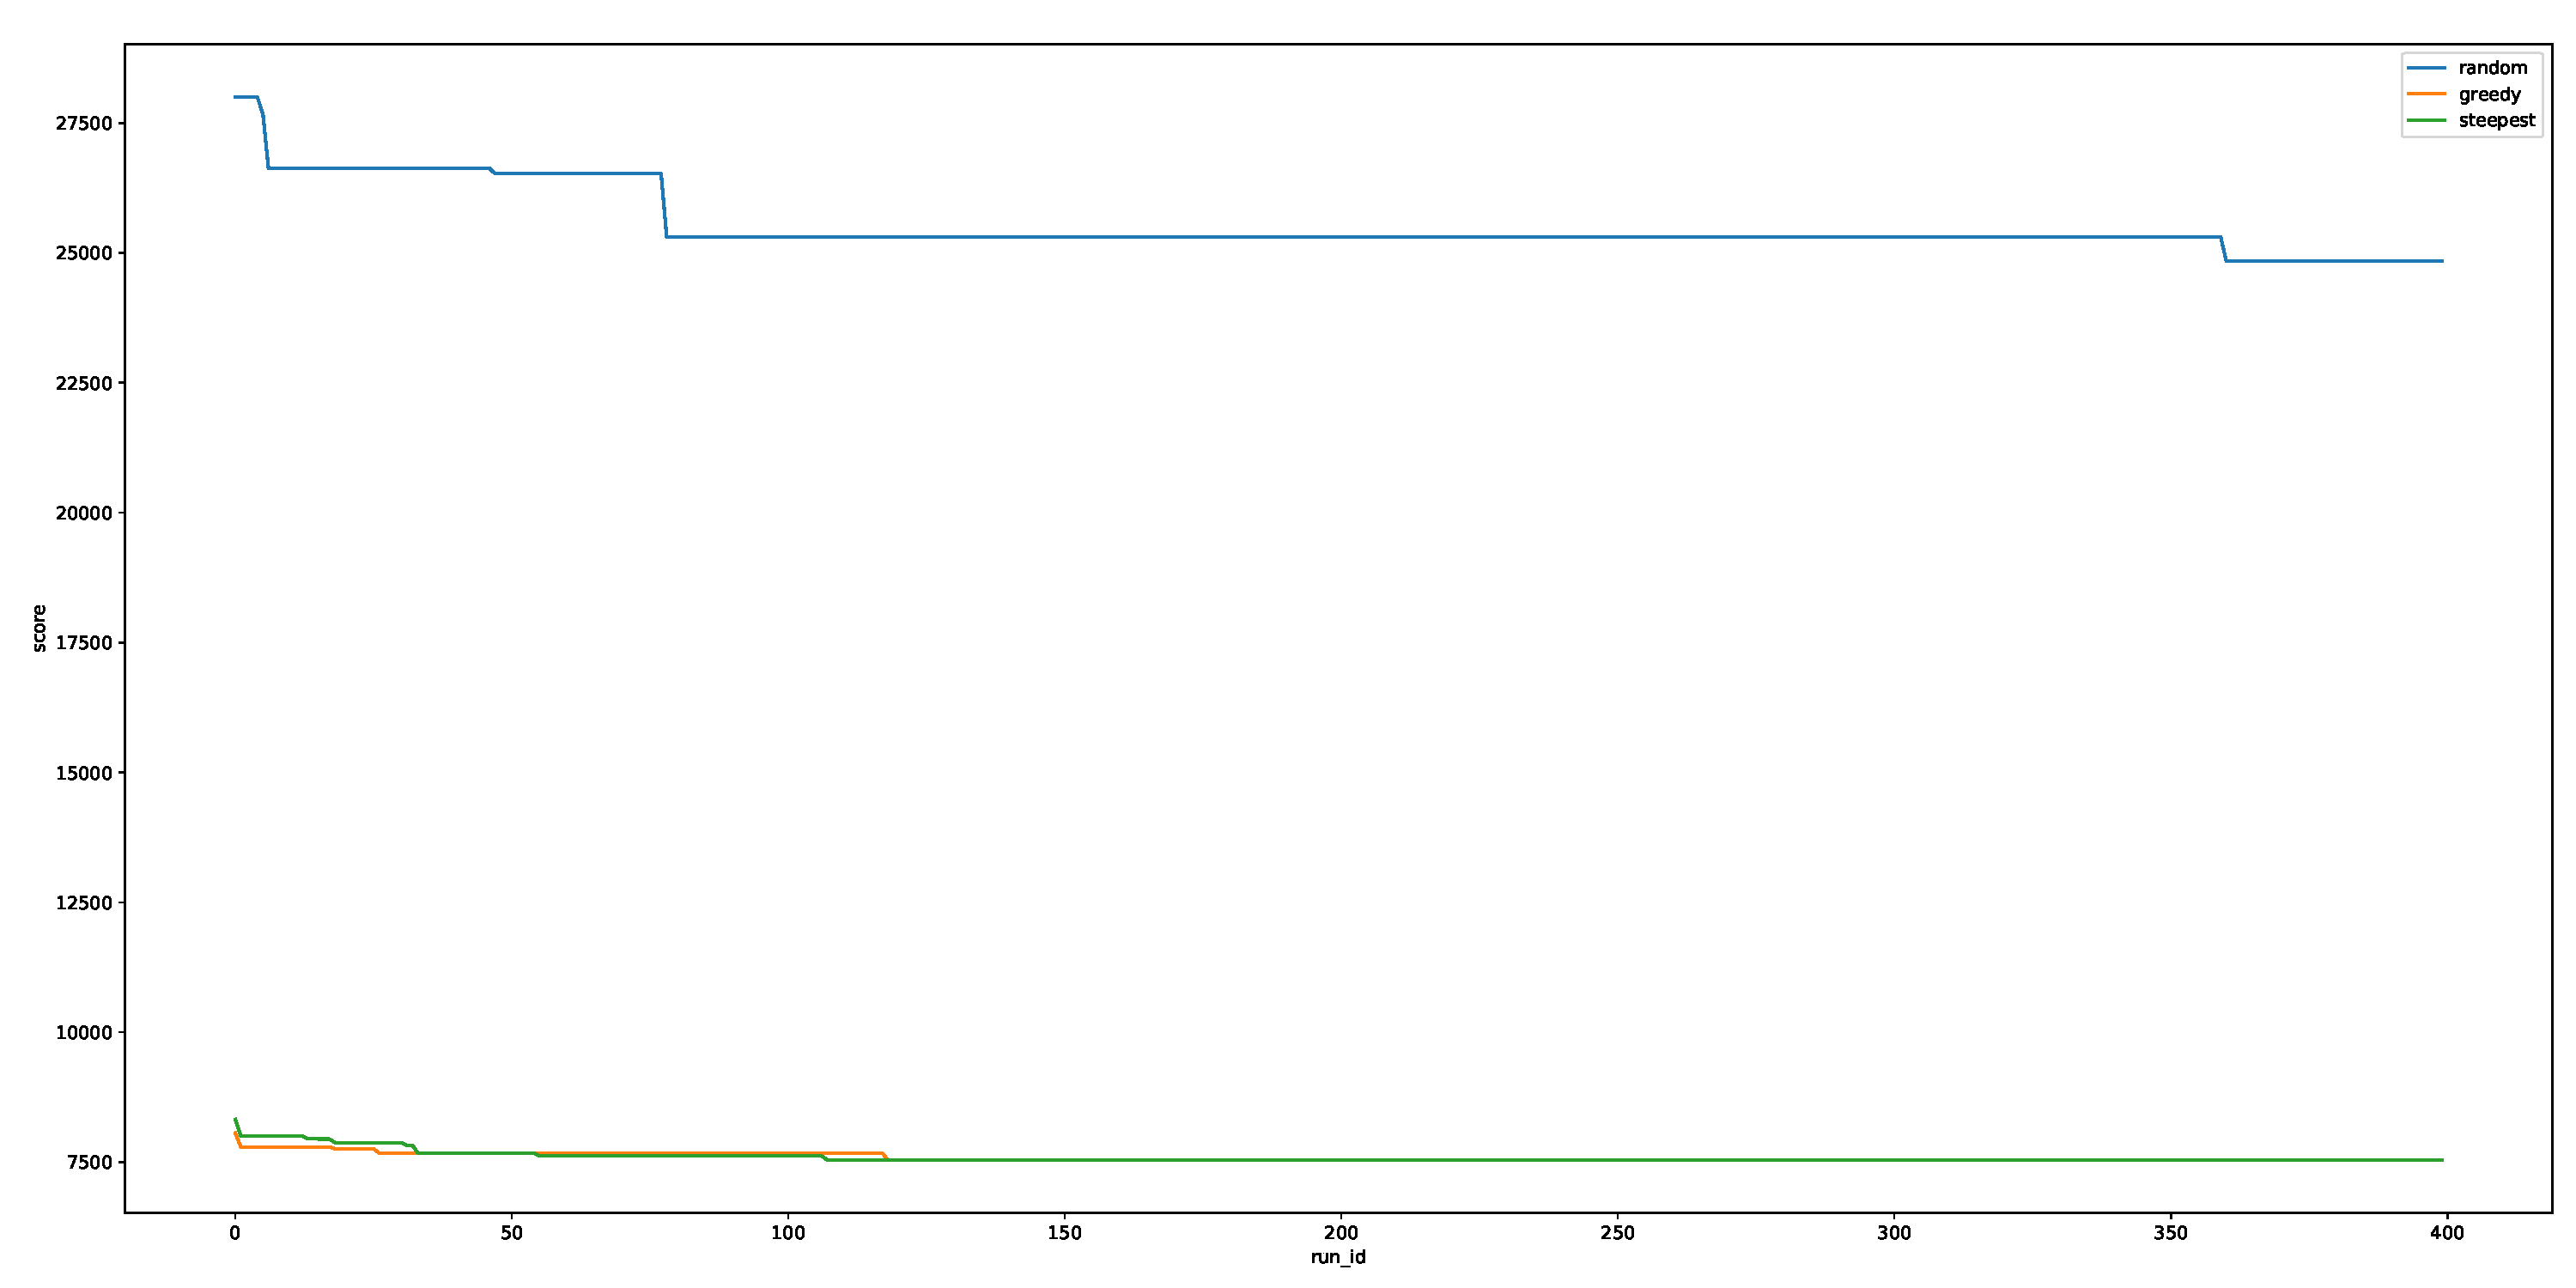
\includegraphics[width=1.0\textwidth]{graphs/multi_start_scoreberlin52.pdf}
\end{center}
\caption{Porównanie jakości rozwiązań algorytmów Gready Search i~Steepest w~zależności od~liczby uruchomień tych algorytmów dla~różnych rozwiązań początkowych dla~zbioru berlin52.}
\label{fig:more_berlin}
\end{figure}

\begin{figure}
\begin{center}
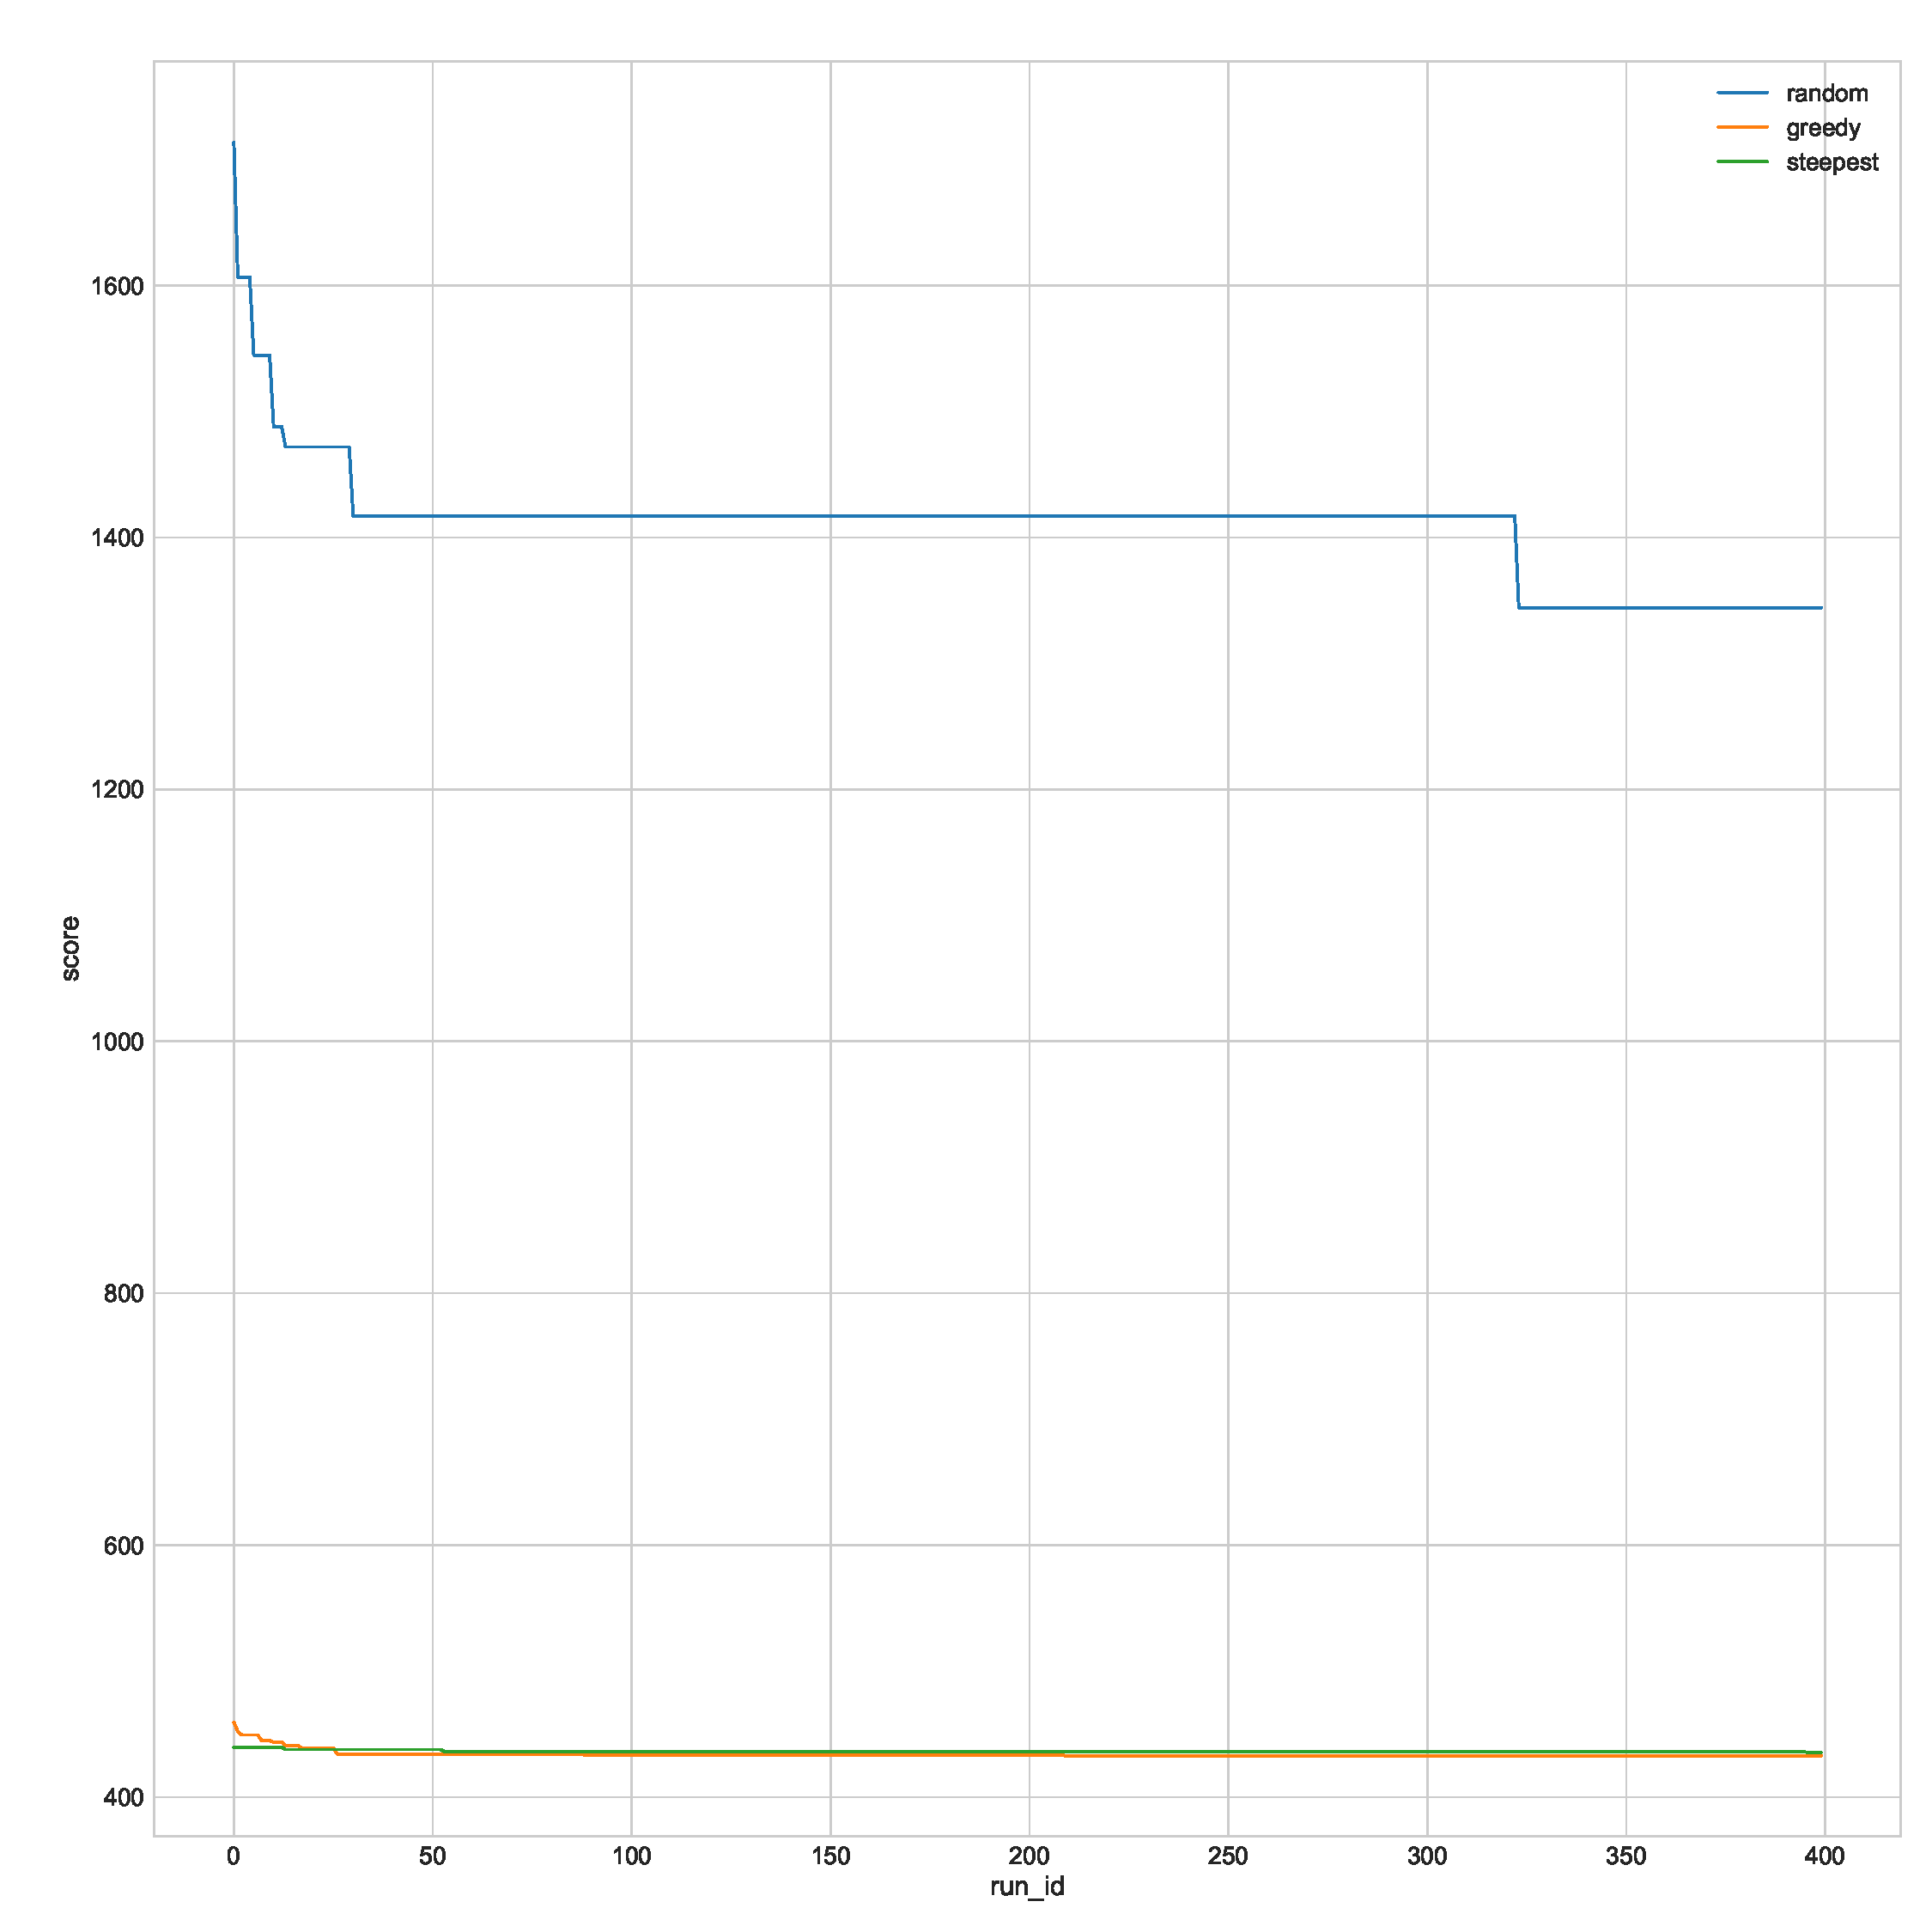
\includegraphics[width=1.0\textwidth]{graphs/multi_start_scoreeil51.pdf}
\end{center}
\caption{Porównanie jakości rozwiązań algorytmów Gready Search i~Steepest w~zależności od~liczby uruchomień tych algorytmów dla~różnych rozwiązań początkowych dla~zbioru eil51.}
\label{fig:more_eil}
\end{figure}

\subsection{Porównanie rozwiązań}

\subsubsection{Miara odległości rozwiązań od rozwiązania optymalnego}

Aby~porównywać między sobą rozwiązania, postanowiliśmy badać, jak~wiele mają takich samych krawędzi. Aby~to~zmierzyć, dla~każdej krawędzi w~jednym rozwiązaniu, sprawdzamy, czy~istnieje ona~w~drugim (skierowana w~dowolną stronę, ponieważ obie krawędzie są~symetryczne).

\subsubsection{Wyniki}

Na~rysunku~\ref{fig:sim} można zaobserwować podobieństwo rozwiązań znajdowanych przez algorytmy do~rozwiązania optymalnego. Istnieje wyraźna zależność polegająca na~tym, że~im~lepsze rozwiązanie, tym~jest~bardziej podobne do~optymalnego.

Bardzo mocno wyróżnia się chmura rozwiązań losowych --- jakość rozwiązań jest~bardzo różnorodna, ale~wszystkie są~bardzo mało podobne do~rozwiązania optymalnego (poniżej 10\%, a~im~więcej miast w~instancji, tym~mniej podobne).

\begin{figure}
\begin{center}
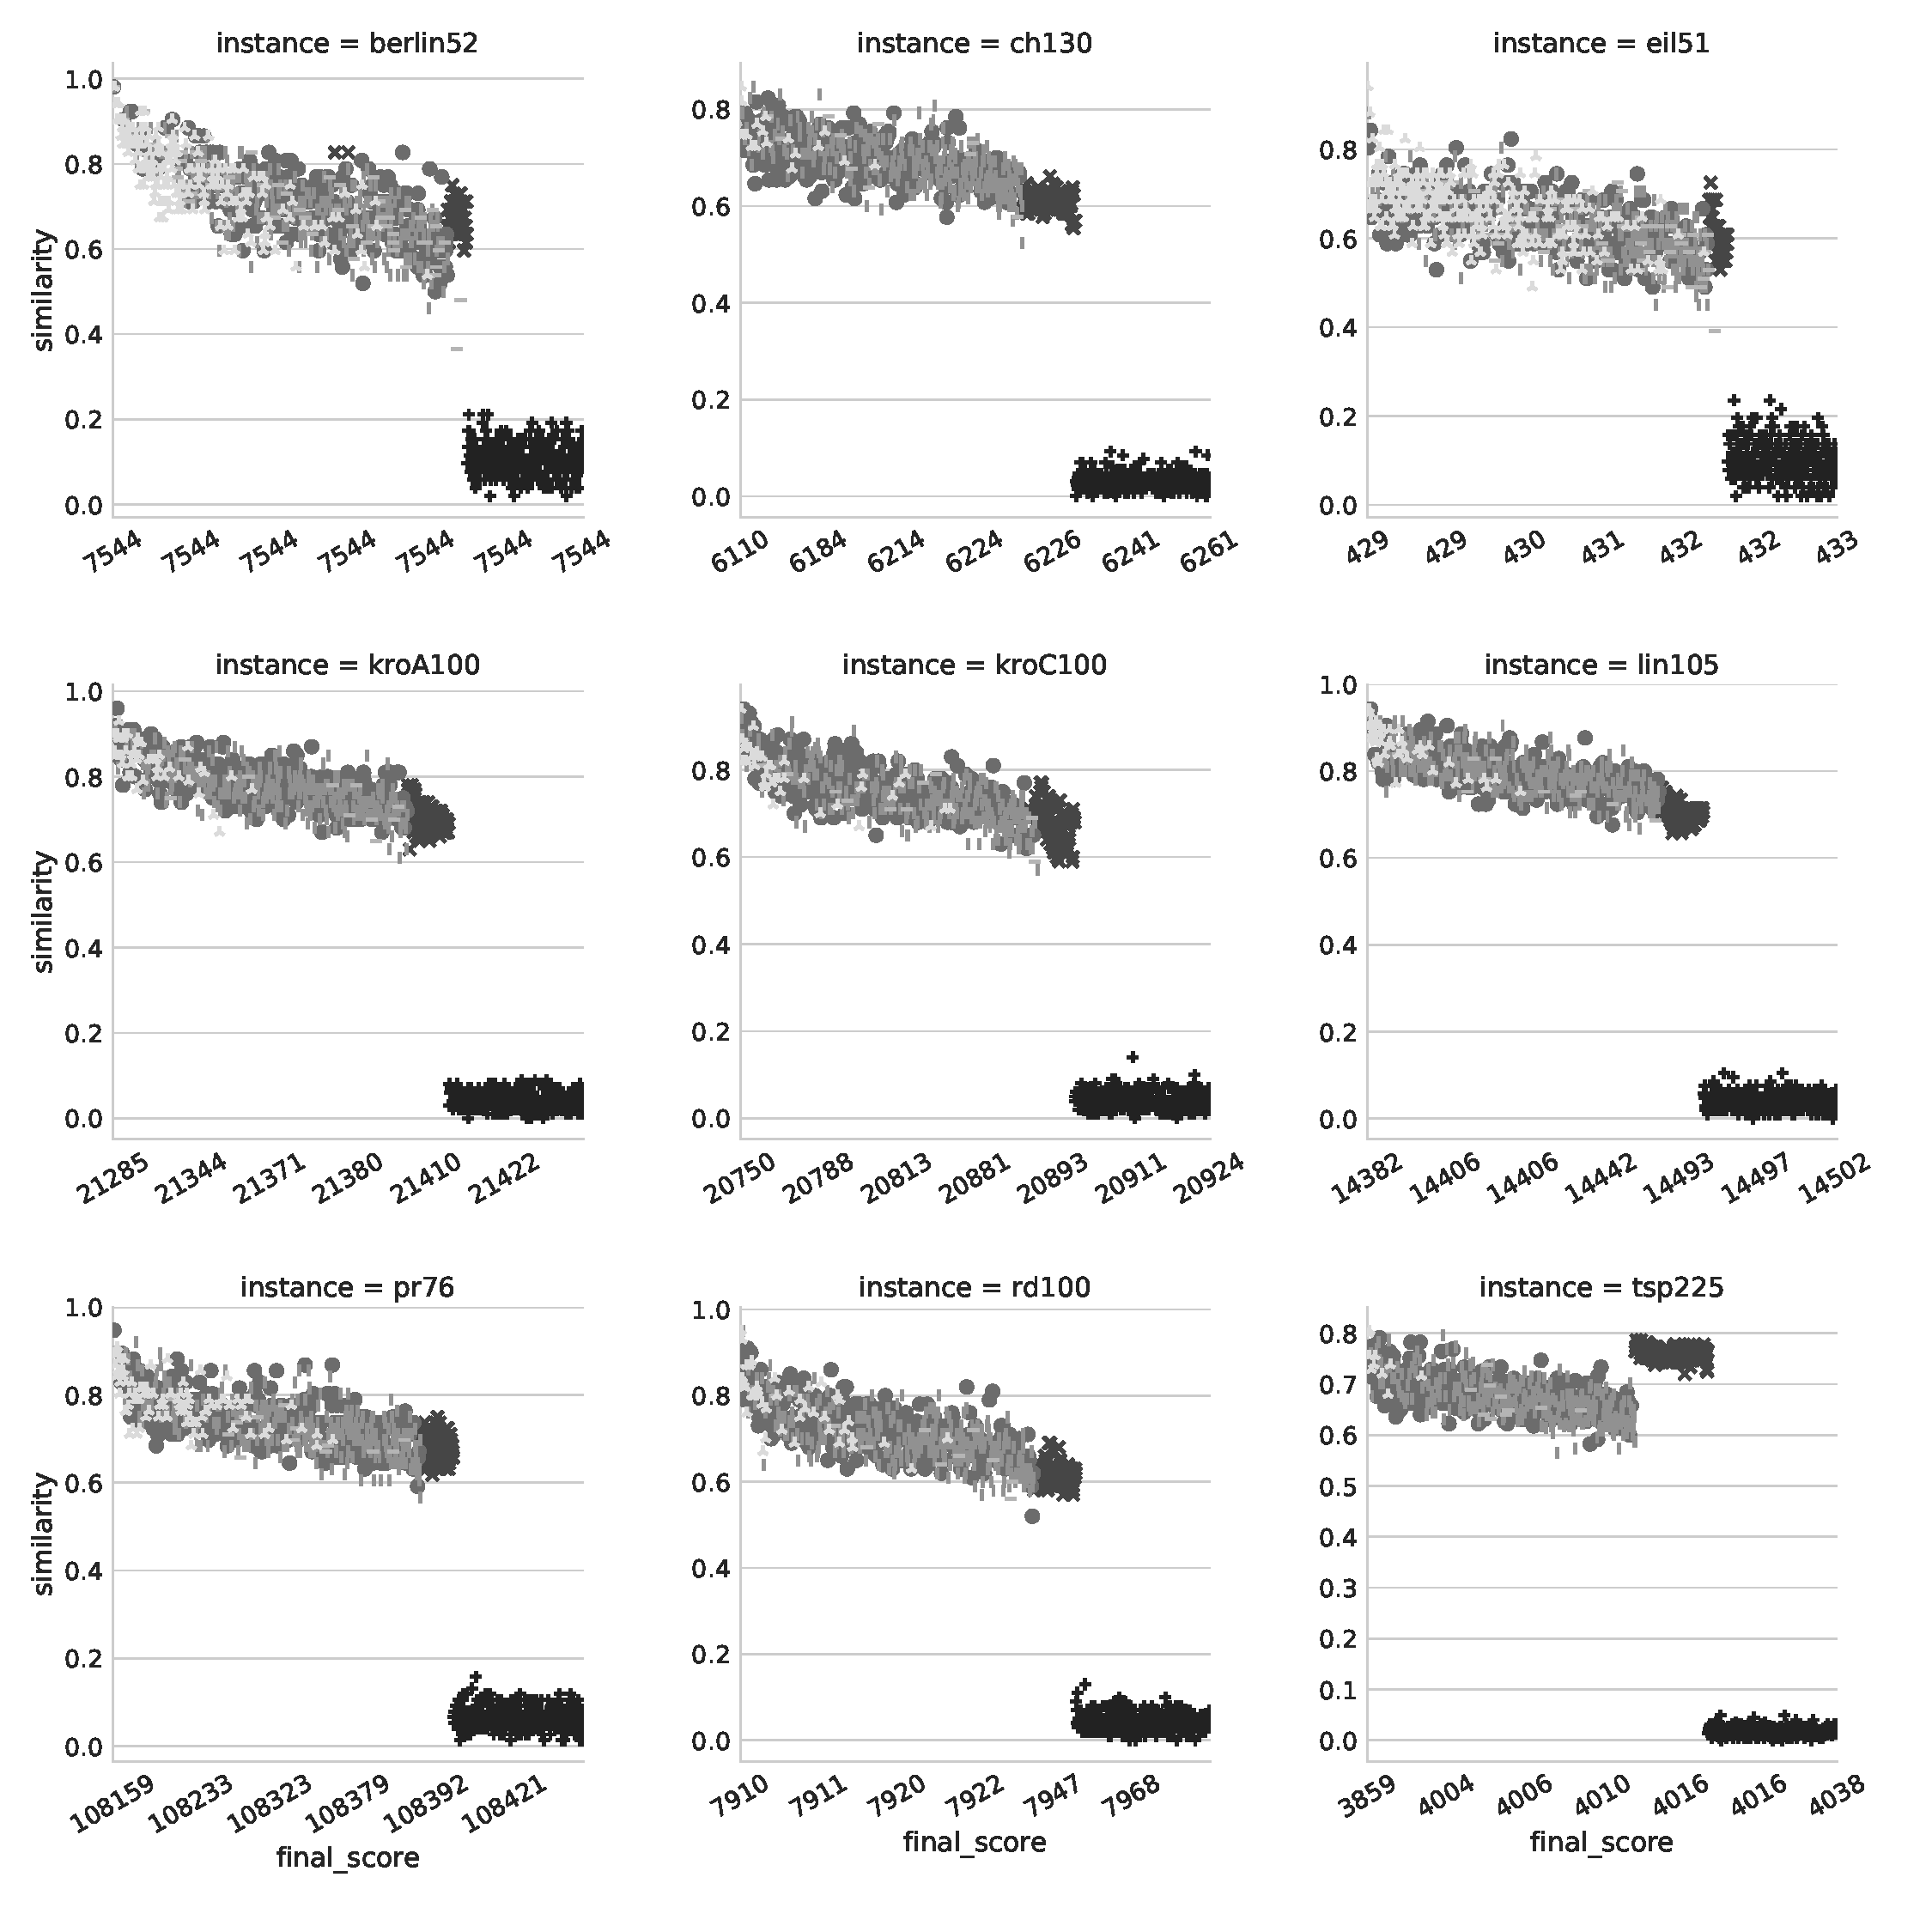
\includegraphics[width=1.0\textwidth]{graphs/similarity_comparision.pdf}
\end{center}
\caption{Porównanie odległości znajdowanych rozwiązań przez algorytmy od~rozwiązania optymalnego.}
\label{fig:sim}
\end{figure}